In Chapter~\ref{chp_soewald2d}, we introduced an efficient algorithm, the SOEwald2D method, to compute the electrostatic energy and force of a quasi-2D system in a homogeneous dielectric medium.
However, in most of the practical applications, the system is confined by dielectric interfaces, which is a more challenging problem.
In this chapter, we focus on the case of dielectrically confined Coulomb systems.
First, we derive the accurate error estimates for the Ewald summation for dielectrically confined Coulomb systems.
Then, we introduce the Random Batch Ewald2D (RBE2D) method, which is a fast and accurate method for computing the electrostatic energy and force of dielectrically confined Coulomb systems.


\section{Accurate error estimates in Ewald summation for dielectrically confined Coulomb systems}

In this section, we present a comprehensive error analysis for both energy and force calculations, addressing the truncation error of the image charge series and the errors arising from the reformulation of the ICM-Ewald2D summation. 
We also perform extensive numerical experiments to validate our error analysis.
We will focus on force-related results in the main text, while energy-related findings are provided in Section~\ref{sec:numeric_energy}.
It is also important to note that in practical computations, the use of FFT can introduce additional errors due to particle spreading onto the uniform grid and the finite resolution of the grid. 
Since these error sources have been thoroughly analyzed in the literature~\cite{deserno1998mesh,wang2012numerical,liang2023error,wang2016multiple,barnett2019parallel,barnett2021aliasing} and are separable from the error discussed in this work, we refer interested readers to these works for more details.

\subsection{Truncation error of the image charge series}\label{sec:error_image}

In this subsection, we analyze the error introduced by truncating the infinite series of image charges at the $M$-th layer. 
This is achieved by reformulating the summation of the infinite image charge series as a Fourier expansion in the periodic $xy$ dimensions and as a geometric series in $z$. 

First, 
let $f(\bm r)$ be a smooth function for $\bm r\in\mathbb R^3$ which decays at infinity, with its Fourier transform denoted as $\widetilde{f}$, then we define the \emph{doubly-periodization} of $f$ as the following lattice sum:
\begin{equation}
f_{\mathcal M} (\bm r)=\sum_{\boldsymbol{m}\in\mathbb{Z}^2} f(\boldsymbol{r}+\V{L}_{\bm{m}})\;,
\end{equation}
and one has the following Poisson summation formula for $f_{\mathcal M} (\bm r)$:
\begin{equation}\label{eq:poissonsum}
f_{\mathcal M} (\bm r)=\frac{1}{2 \pi L_x L_y} \sum_{\bm{k}_{\bm{\rho}}} \int_{\mathbb{R}} \tilde{f}(\bm{k}_{\bm{\rho}}, k_z) e^{\i \bm{k}_{\bm{\rho}} \cdot \boldsymbol{\rho}} e^{\i k_z z} d k_z,
\end{equation}
where $\bm{r}=(\bm{\rho},z)$ with $\bm{\rho}:=(x,y)$, and $\bm{k}_{\bm{\rho}}=2\pi(n_x/L_x,n_y/L_y)$ with $n_x,n_y\in\mathbb{Z}$. 
Applying the Poisson summation formula Eq.~\eqref{eq:poissonsum} to Eq.~\eqref{eq:U_direct} yields 
\begin{equation}\label{eq::33}
    \begin{split}
        U = & \frac{1}{2}\sum_{i,j=1}^{N}q_iq_j\sum_{\bm{m}}{}^\prime\frac{1}{\left|\bm{r}_{ij}+\V{L}_{\bm{m}}\right|} \\
        & + \frac{\pi}{L_xL_y}\sum_{i,j=1}^{N}q_iq_j\sum_{\bm{h}\neq \bm{0}}\frac{e^{-\i \bm{h}\cdot\bm{r}_{ij}}}{h}  \sum\limits_{l=1}^{\infty}\left[\gamma_+^{(l)}e^{-h\left|z_i-z_{j+}^{(l)}\right|}+\gamma_-^{(l)}e^{-h\left|z_i-z_{j-}^{(l)}\right|}\right] \;,
    \end{split}
\end{equation}
where the first term represents the Coulomb energy of a homogeneous quasi-2D system and the second term accounts for the contribution from the image charges. Note that the contribution of the $\bm{h}=\bm{0}$ mode is contained in the homogeneous term, not relevant in the error analysis here for the image charge series.
Now if the image charge series is truncated at the $M$-th layer, then the discarded truncation error term is given by
\begin{equation}\label{eq:trucation_error}
U_{\text{err}}=\frac{\pi}{L_xL_y}\sum_{i,j=1}^{N}q_iq_j\sum_{\bm{h}\neq \bm{0}}\frac{e^{-\i \bm{h}\cdot\bm{r}_{ij}}}{h}\mathcal{G}_{M}(z_i,z_j)\;,  %
\end{equation}
where 
\begin{equation}\label{eq::rGrrij}
 \begin{split}
        \mathcal{G}_{M}(z_i,z_j)&:=\sum\limits_{l=M+1}^{\infty}\left[\gamma_+^{(l)}e^{-h\left|z_i-z_{j+}^{(l)}\right|}+\gamma_-^{(l)}e^{-h\left|z_i-z_{j-}^{(l)}\right|}\right]\; \\
        &= \sum\limits_{l = M + 1}^{\infty} \left[ \gamma_{\T u}^{\lfloor \frac{l}{2} \rfloor}\gamma_{\T d}^{\lceil \frac{l}{2} \rceil} e^{-h (2 \lceil \frac{l}{2} \rceil H + (-1)^l z_i - z_j)} + \gamma_{\T u}^{\lceil \frac{l}{2} \rceil}\gamma_{\T d}^{\lfloor \frac{l}{2} \rfloor} e^{-h (2 \lfloor \frac{l}{2} \rfloor H - (-1)^l z_i + z_j)} \right]\;.
    \end{split}
\end{equation}

To estimate $U_{\text{err}}$, we use the fact that $\mathcal{G}_{M}(z_i,z_j)$ can be reformulated as a geometric series. By inserting the definitions of $\gamma_{\pm}^{(l)}$ and $z_{j \pm}^{(l)}$ into Eq.~\eqref{eq::rGrrij}, we obtain 

\begin{equation}
    \begin{split}
        \mathcal{G}_{M}(z_i,z_j) = & \sum_{n = \frac{M + 1}{2}}^{\infty} \gamma_{\T u}^n \gamma_{\T d}^n e^{-2nhH} \left[ e^{- h z_{ij}} + e^{h z_{ij}} + \gamma_{\T u} e^{- h (z_i + z_j)} + \gamma_{\T d} e^{- h (2 H  - z_i - z_j)}\right] \\
        %= & (\gamma_{\T u} \gamma_{\T d})^{\frac{M + 1}{2}} e^{- (M +1) H h} \sum_{n = 0}^{\infty} \left( \gamma_{\T u} \gamma_{\T d} e^{- 2hH} \right)^n \left[ e^{-h z_{ij}} + e^{h z_{ij}} + \gamma_{\T d} e^{- h (2 H - z_i - z_j)} + \gamma_{\T u} e^{- h (z_i + z_j)} \right] \\
        = & (\gamma_{\T u} \gamma_{\T d})^{\frac{M + 1}{2}} e^{- (M +1) H h} \frac{\left[e^{-h z_{ij}} + e^{h z_{ij}} + \gamma_{\T u} e^{- h (z_i + z_j)} + \gamma_{\T d} e^{- h (2 H - z_i - z_j)} \right] }{1 - \gamma_{\T u} \gamma_{\T d} e^{-2hH}} \;,
    \end{split}
\end{equation}
for odd $M$, and 
\begin{equation}
    \begin{split}
        & \mathcal{G}_M(z_i,z_j) \\
        = & \sum_{n = \frac{M}{2}}^{\infty}  \gamma_{\T u}^n \gamma_{\T d}^n e^{- 2nhH} \left[  \gamma_{\T u} \gamma_{\T d} e^{- h (2 H  + z_{ij})} + \gamma_{\T u} \gamma_{\T d}  e^{- h (2 H  - z_{ij})} + \gamma_{\T u} e^{- h (z_i + z_j)} + \gamma_{\T d} e^{- h (2H  - z_i - z_j)} \right] \\
        = & (\gamma_{\T u} \gamma_{\T d})^{\frac{M}{2}} e^{- M H h} \frac{\left[ \gamma_{\T u} \gamma_{\T d} e^{- h (2 H + z_{ij})} + \gamma_{\T u} \gamma_{\T d} e^{- h (2H - z_{ij})} + \gamma_{\T u} e^{ - h (z_i + z_j)} + \gamma_{\T d} e^{-h (2 H - z_i - z_j)} \right]}{1 - \gamma_{\T u} \gamma_{\T d} e^{-2hH}}  \;,
    \end{split}
\end{equation}
for even $M$. In both cases, we obtain the following error bound:
\begin{equation}\label{eq:beta_ij}
    \abs{ \mathcal{G}_{M}(z_i,z_j) } \leq \abs{\gamma_{\T u} \gamma_{\T d} e^{- 2 H h}}^{\lfloor{(M+1)/2}\rfloor} \frac{\abs{\gamma_{\T u}} + \abs{\gamma_{\T d}} + 2 \abs{\gamma_{\T u} \gamma_{\T d}}}{1 - \abs{\gamma_{\T u} \gamma_{\T d}} e^{-2hH}} \leq \frac{4 \abs{\gamma_{\T u} \gamma_{\T d} e^{- 2 H h}}^{\lfloor{(M+1)/2}\rfloor}}{1 - \abs{\gamma_{\T u} \gamma_{\T d}} e^{-2hH}} \;,
\end{equation}
where we use the fact that 
\begin{equation}
    \begin{split}
        & ~ \abs{\gamma_{\T u} \gamma_{\T d}} e^{-h(2 H + z_{ij})} + \abs{\gamma_{\T u} \gamma_{\T d}} e^{ - h (2 H - z_{ij})} + \abs{\gamma_{\T d}} e^{- h (2 H - z_i - z_j)} + \abs{\gamma_{\T u}} e^{- h (z_i + z_j)} \\
        \leq & ~ 2 \abs{\gamma_{\T u} \gamma_{\T d}} +\abs{\gamma_{\T d}} + \abs{\gamma_{\T u}} \leq 4 \;.
    \end{split}
\end{equation}
Substituting Eq.~\eqref{eq:beta_ij} into Eq.~\eqref{eq:trucation_error}, we have

\begin{equation}\label{eq:U_gamma_bound}
    \begin{split}
        \left|U_{\text{err}}\right| & \leq \frac{4 \pi}{L_x L_y}  \sum_{\bm{h}\neq \bm{0}}  \frac{\abs{\gamma_{\T u} \gamma_{\T d} e^{- 2 hH}}^{\lfloor \frac{M + 1}{2} \rfloor}}{h(1 - \abs{\gamma_{\T u} \gamma_{\T d}} e^{- 2hH})}\abs{\sum_{i,j=1}^{N}q_i q_j e^{-\i \bm{h}\cdot\bm{r}_{ij}}} \\
        & \leq \frac{4\pi}{L_x L_y} \frac{C_{q} \abs{\gamma_{\T u} \gamma_{\T d}}^{\lfloor{(M+1)/2}\rfloor}}{1 - \abs{\gamma_{\T u} \gamma_{\T d}} e^{- 4\pi H / \max\{L_x,L_y\}}} \sum_{\bm{h}\neq \bm{0}} \frac{e^{- 2 \lfloor{(M+1)/2}\rfloor hH}}{h}\\
        & \leq \frac{4\pi}{L_x L_y} \frac{C_{q} \abs{\gamma_{\T u} \gamma_{\T d}}^{\lfloor{(M+1)/2}\rfloor}}{1 - \abs{\gamma_{\T u} \gamma_{\T d}} e^{- 4\pi H / \max\{L_x,L_y\}}} \int_{\frac{2\pi}{\max\{L_x,L_y\}}}^{\infty} 2\pi h \frac{e^{- 2 \lfloor{(M+1)/2}\rfloor hH}}{h} \, \mathrm{d}h \\
        & = \frac{8 \pi^2}{L_x L_y} \frac{C_{q} \abs{\gamma_{\T u} \gamma_{\T d}}^{\lfloor{(M+1)/2}\rfloor} e^{-\frac{4 \pi H \lfloor{(M+1)/2}\rfloor}{\max\{L_x,L_y\}}}}{1 - \abs{\gamma_{\T u} \gamma_{\T d}} e^{- 4\pi H / \max\{L_x,L_y\}}},
    \end{split}
\end{equation}
where $C_q$ is the bound of $|\sum_{i,j}q_iq_je^{-\i \bm{h}\cdot\bm{r}_{ij}}|$, which depends on the charge distribution of the system. 
A rough bound is $C_q\leq \sum_{i,j}|q_iq_j|\leq N^2q_{\text{max}}^2$, where $q_{\text{max}}=\max_{i}|q_i|$ denotes the maximum strength of a single point charge. 
This estimate can be further refined based on prior knowledge of the charge distribution. 
For example, under the Debye-H\"uckel (DH) approximation~\cite{levin2002electrostatic,gan2024fast}, the bound can be tightened to $C_q\leq CNq_{\max}^2$, where $C$ is a constant independent of $N$. 
Either way, we have the following rate of convergence for $|U_{\text{err}}|$ in terms of the truncation parameter $M$:
\begin{equation}\label{eq:Uerr}
|U_{\text{err}}|\sim O\left(\abs{\gamma_{\T u} \gamma_{\T d}}^{\lfloor\frac{M+1}{2}\rfloor} e^{-\frac{4 \pi H \lfloor (M + 1)/2\rfloor}{\max\{L_x,L_y\}}}\right)\;.
\end{equation}

Next, we analyze the truncation error of the force exerted on the $i$-th particle. Using the definition $\bm{F}^i_{\T{err}}=-\nabla_{\bm{r}_i} U_{\text{err}}$ and taking the derivative in each direction, we obtain:
\begin{equation}\label{eq::Ferr}
    \left|\bm{F}^i_{\T{err}}\right| = \left|\nabla_{\bm{r}_i} U_{\text{err}}\right|\leq  \abs{\frac{2\sqrt{3}\pi}{L_xL_y} q_i \sum_{j=1}^{N} q_j\sum_{\bm{h}\neq \bm{0}} e^{-\i \bm{h}\cdot\bm{r}_{ij}}\sum\limits_{l = M + 1}^{\infty}\mathcal{G}_{M}(z_i,z_j)}, 
\end{equation}
where we use the identity $\partial_{z_i}\sum_{ij}\mathcal{G}_M(z_{i},z_{j})=2h\sum_{ij}\mathcal{G}_{M}(z_i,z_j)$, and the factor $\sqrt{3}$ accounts for three dimensions of the force field $\bm F$.  
Substituting Eq.~\eqref{eq:beta_ij} into Eq.~\eqref{eq::Ferr}, we have 
\begin{equation}
\begin{split}
 |F^{i}_{\text{err}}| %& \leq \abs{\frac{2\sqrt{3}\pi}{L_xL_y} q_i \sum_{j=1}^{N} q_j\sum_{\bm{h}\neq \bm{0}} e^{-\i \bm{h}\cdot\bm{r}_{ij}}\sum\limits_{l = M + 1}^{\infty}\mathcal{G}_{M}(z_i,z_j)}\\
 & \leq \frac{8\sqrt{3}\pi}{L_xL_y}  \frac{C_{Q} \abs{\gamma_{\T u} \gamma_{\T d}}^{\lfloor{(M+1)/2}\rfloor}}{1 - \abs{\gamma_{\T u} \gamma_{\T d}} e^{- 4\pi H / \max\{L_x,L_y\}}} \sum_{\bm{h}\neq \bm{0}} e^{- 2 \lfloor{(M+1)/2}\rfloor hH}\\
 & \leq \frac{8\sqrt{3}\pi}{L_xL_y} \frac{ C_Q\abs{\gamma_{\T u} \gamma_{\T d}}^{\lfloor{(M+1)/2}\rfloor}}{1 - \abs{\gamma_{\T u} \gamma_{\T d}} e^{- 4\pi H / \max\{L_x,L_y\}}} \int_{\frac{2\pi}{\max\{L_x,L_y\}}}^{\infty} 2\pi h e^{- 2 \lfloor{(M+1)/2}\rfloor hH} \, \mathrm{d}h \\
& = \frac{16\sqrt{3} \pi^2}{L_xL_y} \frac{C_Q \abs{\gamma_{\T u} \gamma_{\T d}}^{\lfloor{(M+1)/2}\rfloor}}{1 - \abs{\gamma_{\T u} \gamma_{\T d}} e^{- 4\pi H / \max\{L_x,L_y\}}}  \frac{\left[1 + \frac{2\pi \lfloor{(M+1)/2}\rfloor H}{\max\{L_x,L_y\}}\right]}{4 \lfloor{(M+1)/2}\rfloor^2 H^2} e^{- \frac{4\pi \lfloor{(M+1)/2}\rfloor H}{\max\{L_x,L_y\}}}\;,
\end{split}
\end{equation}
where the second inequality is derived from the monotonicity of the exponential function, and $C_Q=|q_{i}\sum_{j=1}^{N}q_je^{-\i\bm{h}\cdot \bm{r}_{ij}}|\leq Nq_{\text{max}}^2$. 
If the DH theory is applied, the prefactor $C_Q$ can be further tightened to $C_Q\leq Cq_{\max}^2$, where $C$ is a constant independent of $N$. 
Similarly, considering the rate of convergence in terms of $M$, we have
\begin{equation}\label{eq::Ferr1}
|\bm{F}^i_{\text{err}}| \sim O\left(\lfloor (M+1)/2\rfloor^{-1}\abs{\gamma_{\T u} \gamma_{\T d}}^{\lfloor\frac{M+1}{2}\rfloor} e^{-\frac{4\pi H \lfloor(M+1)/2\rfloor}{\max\{L_x,L_y\}}}\right)\;.
\end{equation}
Comparing Eq.~\eqref{eq::Ferr1} and Eq.~\eqref{eq:Uerr},
we observed that the error in force converge slightly faster than that of the energy by a factor of $\lfloor (M+1)/2\rfloor^{-1}$. 

To validate our theoretical predictions, we employ the ICM-Ewald2D summation (i.e., Eqs.~\eqref{eq::Uc} and~\eqref{eq::Fourier2D}) to calculate the relative errors in force, $\mathcal{E}_r = \max\limits_{i=1,\ldots,N}\frac{\abs{\bm{F}^i_{\text{err}}}}{\abs{\bm{F}^i}}$, as a function of $M$, the number of truncated image layers.
Without loss of generality, we examine charge-asymmetric systems containing $13$ divalent cations and $26$ monovalent anions, randomly distributed within the simulation cell. 
In all calculations, the dimensions of the simulation cell along the periodic directions are fixed as $L_x = L_y = 10$, while the aspect ratio of the system is adjusted by varying the cell height $H$. 
Recall that the reflection factors for the upper and lower dielectric interfaces are denoted as $\gamma_{\T u}$ and $\gamma_{\T d}$, respectively. 
Finally, unless otherwise specified, we always set the Ewald splitting parameter $s=6$ to ensure that the errors due to Ewald decomposition remain negligible. 



The numerical results are presented in Fig.~\ref{fig:icm_error_force} (a) and (b), where we examine the convergence rate of $\mathcal{E}_r$ under different aspect ratios $L_x / H$ and reflection factors $\gamma=\gamma_{\T u}=\gamma_{\T d}$, respectively.
All results demonstrate that the force errors decay exponentially as $M$ increases. 
Additionally, we observe that the errors decay slower as the aspect ratio $L_x / H$ (Fig.~\ref{fig:icm_error_force} (a)) and the reflection factor $\gamma$ (Fig.~\ref{fig:icm_error_force} (b)) increases, both are consistent with our theoretical predictions in Eq.~\eqref{eq::Ferr1}. 
Furthermore, to quantitatively validate our theoretical findings, we also plot the theoretical decay rates predicted by Eq.~\eqref{eq::Ferr1} as dashed lines in Fig.~\ref{fig:icm_error_force}, showing excellent agreement with our numerical results.
The results for relative errors in energy are documented in Section~\ref{sec:numeric_energy}, where similar conclusions hold.  

%In \Cref{fig:icm_error_force} (a) and (b), we maintained fixed values for the reflection rate and the system height, respectively. 
%The results indicate that the energy error decreases exponentially with the number of reflection levels, denoted as~$M$, and the speed of decay depends on the reflection rate $\gamma$ and the system height $H$.
%The inset illustrates that the slope of the fitting line corresponds to the theoretical value $\lg(\gamma e^{-2\pi H / L_x})$, aligning with the theoretical prediction in Eq.~\eqref{eq:F_gamma_bound}.
%Additionally, the results on the energy error are presented in the Section 1 of supporting information.

\begin{figure}[htbp]
    \centering
    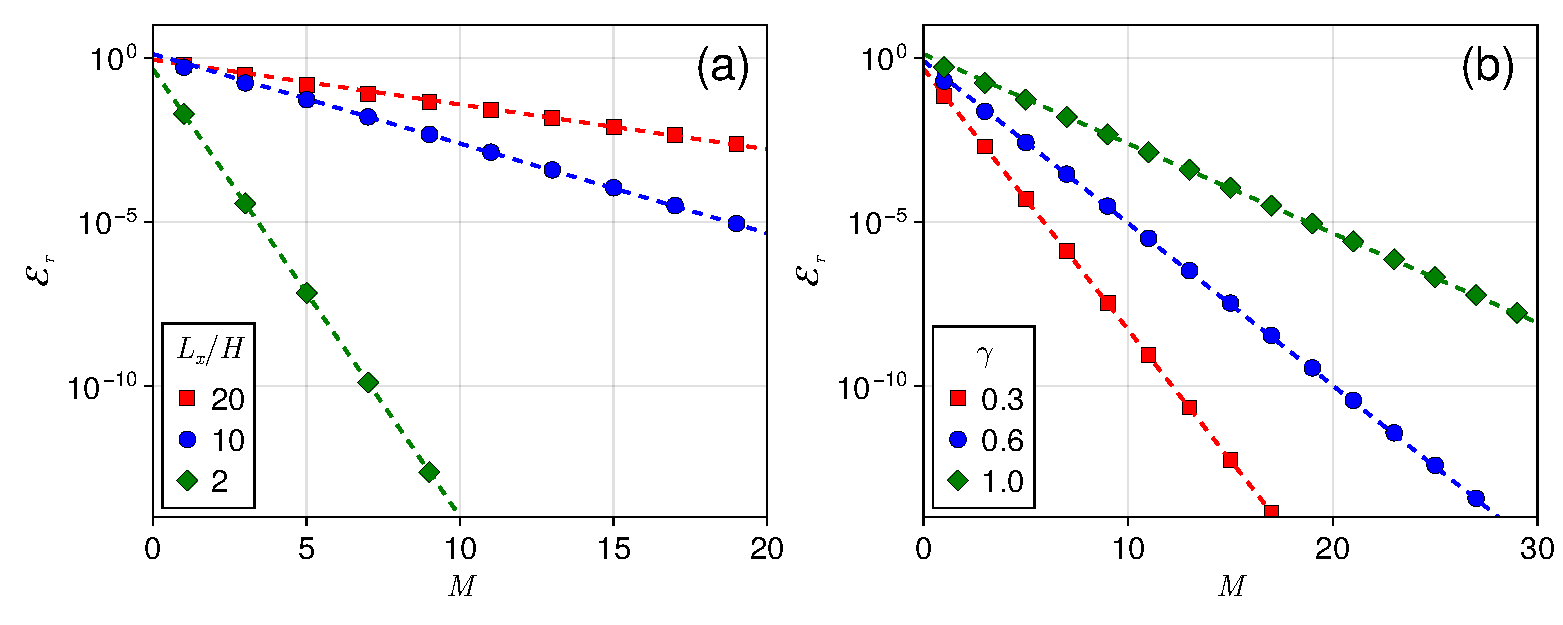
\includegraphics[width=0.98\linewidth]{figs/icm_error_force.pdf}
    \caption{
        Relative errors in force ($\mathcal{E}_r$) as a function of the truncation parameter $M$ for the image charge series. 
        The dashed lines represent the fitted curves with decay rates using our theoretical prediction Eq.~\eqref{eq::Ferr1}. 
        In panel (a), we fix $\gamma_{\T u} = \gamma_{\T d} = 1$ and consider systems with varying heights $H = 0.5$, $1$, and $5$. In panel (b), we fix $H = 1$ while varying $\gamma_{\T u} = \gamma_{\T d} = \gamma$ with values of $0.3, 0.6,$ and $1$. In both panels, we fix $L_x=L_y=10$.
    }
    \label{fig:icm_error_force}
\end{figure}

\subsection{Estimations of electrostatic layer correction (ELC) with image charges}\label{sec:error_reform}

Another often-overlooked source of error in existing algorithms stems from the omission of the ELC term in Eq.~\eqref{eq:U^M_ELC} and the discretization error using the trapezoidal rule, which has been discussed in Section~\ref{sec::icm_ewald2d}. 
In this section, we focus on deriving estimations of the ELC term with image charges.
%a rough estimation has been given as the following Lemma~\cite{gan2024fast}.

First, we recall the definition of the ELC term with image charges, denoted as $U_{\text{ELC}}^{M}$, as provided in the energy expressions Eqs.~\eqref{eq:U^M_ELC} and~\eqref{eq::23}:
\begin{equation}\label{eq::UELCm}
U_{\T {ELC}}^{M}:=\frac{2\pi}{L_xL_y}\sum_{i,j=1}^{N}q_iq_j\sum_{\bm{h}\neq \bm{0}} \frac{e^{\i \bm{h}\cdot\bm{r}_{ij}}e^{-hL_z}\left[\cosh(hz_{ij})+\mathscr{F}_{\text{ELC}}^{M}(z_i,z_j)\right]}{h(e^{-hL_z}-1)}\;.
\end{equation}
To derive an estimation for $U_{\T {ELC}}^{M}$, we introduce the following two inequalities. 
1). By basic algebraic manipulations, one obtains:  
\begin{equation}\label{eq::bpud1}
e^{-hL_z}\cosh(hz_{ij})\leq e^{-h(L_z-|z_{ij}|)}\leq e^{-h(L_z-H)}\;,
\end{equation}
and 2).
\begin{equation}\label{eq::bpud2}
\begin{split}
& e^{-hL_z}\mathscr{F}_{\text{ELC}}^{M}(z_i,z_j) \\
= & e^{-hL_z}\sum\limits_{l=1}^{M}\left[\gamma_{+}^{(l)}\cosh(h(z_i-z_{j+}^{(l)}))+\gamma_{-}^{(l)}\cosh(h(z_i-z_{j-}^{(l)}))\right]\\
= & \frac{1}{2}\sum\limits_{l=1}^{M}\left[\gamma_{+}^{(l)}e^{-h(L_z-|z_i-z_{j+}^{(l)}|)}+\gamma_{-}^{(l)}e^{-h(L_z-|z_i-z_{j-}^{(l)}|)}\right]+\frac{e^{-hL_z}}{2}(\mathcal{G}_{0}(z_i,z_j)-\mathcal{G}_{M}(z_i,z_j))\\
\leq & \frac{1}{2}\sum_{l=1}^{M}C^{(l)}_{\gamma}e^{-h(L_z-(l+1)H)}+\frac{(|\gamma_{\T u}|+|\gamma_{\T d}| + 2|\gamma_{\T u}\gamma_{\T d}|)e^{-hL_z}}{1-|\gamma_{\T u}\gamma_{\T d}|e^{-2hH}},
\end{split}
\end{equation}
where the factor $C^{(l)}_{\gamma}$ is defined as 
\begin{equation}
C^{(l)}_{\gamma}:=\left|\gamma_{+}^{(l)}\right|+\left|\gamma_{-}^{(l)}\right|=\left| \gamma_{\T d}^{\lceil l/2 \rceil} \gamma_{\T u}^{\lfloor l/2 \rfloor}\right|+\left| \gamma_{\T d}^{\lfloor l/2 \rfloor} \gamma_{\T u}^{\lceil l/2 \rceil}\right|.
\end{equation}
To obtain the above inequality, we use the definitions of $\gamma_{+}^{(l)}$ and $\gamma_{-}^{(l)}$, the bound $\max_{i,j}\{|z_i-z_{j+}^{(l)}|,|z_i-z_{j-}^{(l)}|\}\leq (l+1)H$, and the definition of $\mathcal{G}_{M}(z_i,z_j)$ in Eq.~\eqref{eq::rGrrij} along with its bound given in Eq.~\eqref{eq:beta_ij}. 
Substituting Eqs.~\eqref{eq::bpud1} and \eqref{eq::bpud2} into Eq.~\eqref{eq::UELCm} yields

\begin{equation}
\resizebox{.98\hsize}{!}{$
\begin{split}
\left|U_{\text{ELC}}^{M}\right|&\leq \frac{2\pi}{L_xL_y}\sum_{\bm{h}\neq \bm{0}} \frac{C_q\left[e^{-h(L_z-H)}+\frac{1}{2}\sum\limits_{l=1}^{M}C^{(l)}_{\gamma}e^{-h(L_z-(l+1)H)}+\frac{(|\gamma_{\T u}|+|\gamma_{\T d}| + 2|\gamma_{\T u}\gamma_{\T d}|)e^{-hL_z}}{1-|\gamma_{\T u}\gamma_{\T d}|e^{-\frac{4\pi H}{\max\{L_x,L_y\}}}}\right]}{h(1-e^{-\frac{2\pi L_z}{\max\{L_x,L_y\}}})}\\
&\leq \frac{4\pi^2 C_q}{L_xL_y(1-e^{-\frac{2\pi L_z}{\max\{L_x,L_y\}}})}\int^{\infty}_{\frac{2\pi}{\max\{L_x,L_y\}}} \left[e^{-h(L_z-H)}+\sum\limits_{l=1}^{M}\frac{C^{(l)}_{\gamma}}{2}e^{-h(L_z-(l+1)H)}+\frac{4e^{-hL_z}}{1-e^{-\frac{4\pi H}{\max\{L_x,L_y\}}}}\right]dh\\
&=\frac{4\pi^2 C_q}{L_xL_y(1-e^{-\frac{2\pi L_z}{\max\{L_x,L_y\}}})}\left[\frac{e^{-\frac{2\pi(L_z-H)}{\max\{L_x,L_y\}}}}{L_z-H}+\sum_{l=1}^{M}\frac{C_{\gamma}^{(l)}e^{-\frac{2\pi(L_z-(l+1)H)}{\max\{L_x,L_y\}}}}{2(L_z-(l+1)H)}+\frac{4e^{-\frac{2\pi L_z}{\max\{L_x,L_y\}}}}{L_z(1-e^{-\frac{4\pi H}{\max\{L_x,L_y\}}})} \right],
\end{split}
$}
\end{equation}
where we recall $C_q$ is the bound of $|\sum_{i,j=1}^{N}q_iq_je^{\i \bm{h}\cdot\bm{r}_{ij}}|$, $\left|\gamma_{\T u}\right|\leq 1$, and $\left|\gamma_{\T d}\right|\leq 1$. 
Finally, suppose $L_z>(M+1)H$, we obtain the following estimation for the ELC contribution in energy, $U_{\text{ELC}}^{M}$, as:
\begin{equation}
\label{eq::U_ELC}
\left|U_{\text{ELC}}^{M}\right|\sim O\left(e^{-\frac{2\pi(L_z-H)}{\max\{L_x,L_y\}}}+\sum_{l=1}^{M}C_{\gamma}^{(l)}e^{-\frac{2\pi(L_z-(l+1)H)}{\max\{L_x,L_y\}}}\right).
\end{equation}

The corresponding ELC term in force calculations can be estimated analogously. 
We have
\begin{equation}
\left|\bm{F}_{\text{ELC}}^{M,i}\right|:=|-\nabla_{\bm{r}_i} U_{\text{ELC}}^{M}|\leq \left|\frac{4\sqrt{3}\pi}{L_xL_y}q_i\sum_{j=1}^{N}q_j\sum_{\bm{h}\neq \bm{0}} \frac{e^{\i \bm{h}\cdot\bm{r}_{ij}}e^{-hL_z}\left[\cosh(hz_{ij})+\mathscr{F}_{\text{ELC}}^{M}(z_i,z_j)\right]}{1-e^{-hL_z}}\right|\;.
\end{equation}
Further applying the inequalities Eqs.~\eqref{eq::bpud1} and \eqref{eq::bpud2}, we obtain:

\begin{equation}
\resizebox{0.98\hsize}{!}{$
\begin{split}
\left|\bm{F}_{\text{ELC}}^{M,i}\right|\leq &\frac{4\sqrt{3}\pi}{L_xL_y}\sum_{\bm{h}\neq \bm{0}} \frac{C_Q\left[e^{-h(L_z-H)}+\frac{1}{2}\sum\limits_{l=1}^{M}C^{(l)}_{\gamma}e^{-h(L_z-(l+1)H)}+\frac{(|\gamma_{\T u}|+|\gamma_{\T d}| + 2|\gamma_{\T u}\gamma_{\T d}|)e^{-hL_z}}{1-|\gamma_{\T u}\gamma_{\T d}|e^{-\frac{4\pi H}{\max\{L_x,L_y\}}}}\right]}{1-e^{-\frac{2\pi L_z}{\max\{L_x,L_y\}}}}\\
\leq& \frac{8\sqrt{3}\pi^2 C_Q}{L_xL_y(1-e^{-\frac{2\pi L_z}{\max\{L_x,L_y\}}})}\int_{\frac{2\pi}{\max\{L_x,L_y\}}}^{\infty}h\left[e^{-h(L_z-H)}+\frac{1}{2}\sum\limits_{l=1}^{M}C^{(l)}_{\gamma}e^{-h(L_z-(l+1)H)}+\frac{4e^{-hL_z}}{1-e^{-\frac{4\pi H}{\max\{L_x,L_y\}}}}\right]dh\\
=&\frac{8\sqrt{3}\pi^2 C_Q}{L_xL_y(1-J_3)}\left[\frac{1+J_1}{(L_z-H)^2}e^{-J_1}+\sum_{l=1}^{M}\frac{C_{\gamma}^{(l)}(1+J_2^{(l)})}{2(L_z-(l+1)H)^2}e^{-J_2^{(l)}}+\frac{4(1+J_3)}{L_z^2(1-e^{-\frac{4\pi H}{\max\{L_x,L_y\}}})}e^{-J_3}\right]
\end{split}
$}
\end{equation}
where $C_Q$ is the bound of $|q_i\sum_{j=1}^{N}q_je^{-\i \bm{h}\cdot\bm{r}_{ij}}|$ and the coefficients $J_1$, $J_2^{(l)}$ and $J_3$ are defined via
\begin{equation}
J_1=\frac{2\pi(L_z-H)}{\max\{L_x,L_y\}},\quad\; J_2^{(l)}= \frac{2\pi(L_z-(l+1)H)}{\max\{L_x,L_y\}}\quad \;\text{and} \quad \; J_3=\frac{2\pi L_z}{\max\{L_x,L_y\}}.
\end{equation}
As before, by omitting all the prefactors, we arrive at the following estimation for the ELC contribution in force calculations:
\begin{equation}\label{eq::ForceError}
\left|\bm{F}_{\text{ELC}}^{M,i}\right|\sim O\left(e^{-\frac{2\pi(L_z-H)}{\max\{L_x,L_y\}}}+\sum_{l=1}^{M}C_{\gamma}^{(l)}e^{-\frac{2\pi(L_z-(l+1)H)}{\max\{L_x,L_y\}}}\right).
\end{equation}
Clearly, comparing Eq.~\eqref{eq::ForceError} and Eq.~\eqref{eq::U_ELC}, we find that the ELC contribution behaves asymptotically the same for both energy and force calculations.

\subsection{Leading-order analysis of the ELC term and numerical validations}\label{sec::leadingerr}
The theoretical estimations of the ELC term, as presented in Eqs.~\eqref{eq::ForceError} and~\eqref{eq::U_ELC}, behave differently under different system aspect ratios and reflection factors.
In this section, we conduct a detailed analysis of the leading-order contribution of the ELC term across different system parameter scenarios. 
Our focus will be on the analysis of force calculations, a similar approach can be applied to the energy.

First, by introducing two new dimensionless parameters $g_{\T u}:=\gamma_{\T u}e^{\frac{2\pi H}{\max\{L_x,L_y\}}}$ and $g_{\T d}:=\gamma_{\T d}e^{\frac{2\pi H}{\max\{L_x,L_y\}}}$, Eq.~\eqref{eq::ForceError} can be reformulated as
\begin{equation}
   \label{eq::Error_refo}
   \begin{aligned} \left|\bm{F}_{\text{ELC}}^{M,i}\right|&\sim e^{-\frac{2\pi(L_z-H)}{\max\{L_x,L_y\}}} \left[ 1 + \sum_{l=1}^{M} \left( g_{\T u}^{\lfloor \frac{l}{2} \rfloor} g_{\T d}^{\lceil \frac{l}{2} \rceil} + g_{\T u}^{\lceil \frac{l}{2} \rceil} g_{\T d}^{\lfloor \frac{l}{2} \rfloor} \right) \right]\\
   &=e^{-\frac{2\pi(L_z-H)}{\max\{L_x,L_y\}}}\left[(g_{\T u} + g_{\T d} + 2) \sum_{l = 0}^{\lfloor \frac{M - 1}{2} \rfloor} (g_{\T u}g_{\T d})^{l} + ((-1)^{M}+1) (g_{\T u}g_{\T d})^{\lfloor \frac{M}{2} \rfloor} - 1\right]\,.
   \end{aligned}
\end{equation}
From Eq.~\eqref{eq::Error_refo}, it is clear that the leading-order contribution of the ELC term depends on the magnitude of $|g_{\T u}g_{\T d}|$. 
Specifically, i). if $|g_{\T u}g_{\T d}| > 1$, the ELC leading-order term grows exponentially as $M$ increases:
\begin{equation}\label{eq::lhs_bigger1}
   \abs{\V{F}_{\text{ELC}}^{M,i}} =  \left\{
	\begin{aligned}
		& O \left(2 \abs{g_{\T u} g_{\T d}}^{M/2} e^{-\frac{2\pi (L_z - H)}{\max\{L_x,L_y\}}} \right) , & \text{if $M$ is even,}\\
		& O \left( \left(g_{\T u} + g_{\T d}+2\right)\abs{g_{\T u} g_{\T d}}^{\frac{M-1}{2}} e^{-\frac{2\pi (L_z -H)}{\max\{L_x,L_y\}}} \right) , & \text{if $M$ is odd.}
	\end{aligned}
	\right.
\end{equation} 
ii). If $|g_{\T u}g_{\T d}|=1$, the ELC leading-order term grows linearly with $M$:
\begin{equation}
\label{eq::lhs_1}
\abs{\V{F}_{\text{ELC}}^{M,i}} = O \left( \frac{M}{2}\left(g_{\T u} + g_{\T d}+2\right)e^{-\frac{2\pi L_z}{\max\{L_x,L_y\}}} \right)\;.
\end{equation}
iii). If $|g_{\T u}g_{\T d}|<1$, the summation in Eq.~\eqref{eq::Error_refo} converges as $M\rightarrow +\infty$, yielding a uniform estimation independent with $M$:
\begin{equation}
\label{eq::lhs_less1}
\abs{\V{F}_{\text{ELC}}^{M,i}} \sim O \left( \left(g_{\T u}+g_{\T d}+2\right)e^{-\frac{2\pi L_z}{\max\{L_x,L_y\}}} \right).
\end{equation}
The preceding analysis indicates that, for a fixed system size \( L_z \) (including vacuum layers), the numerical error associated with neglecting the ELC term exhibits a non-trivial dependence on the number of image charge layers \( M \). 
Specifically, for \( |g_{\T u}g_{\T d}|>1 \), the error grows exponentially with \( M \);
for \( |g_{\T u}g_{\T d}| = 1 \), it grows linearly; and for \( |g_{\T u}g_{\T d}| < 1 \), no error escalation is observed as \( M \) increases.

In what follows, we perform a series of numerical tests to validate our theoretical analysis. 
First, we examine the simplest case, i.e., systems \emph{without} dielectric interfaces by setting $\gamma_{\T u} = \gamma_{\T d} = 0$. 
In our numerical tests, we fix $L_x = L_y = 10$, and vary the system heights by setting $H = 0.5, 1, 5$. 
For clarity, we further introduce the dimensionless \emph{padding ratio} $R$, defined as $P = (L_z - H) / L_x$. 
The results, presented in Fig.~\ref{fig:elc_error_force}, clearly show that the relative errors in force $\mathcal{E}_r$ decay exponentially with $P$. 
Notably, the convergence with respect to $P$ is independent of the specific choice of $H$, aligning with our theoretical predictions in Eq.~\eqref{eq::ForceError}. 
Furthermore, our findings underscore the computational challenges of simulating \emph{strongly-confined} systems, characterized by a high aspect ratio, i.e., $L_x / H$. 
According to Fig.~\ref{fig:elc_error_force}, achieving single- or double-precision relative accuracy requires padding the system in the $z$ direction such that $(L_z - H)/L_x$ reaches around 3 and 5, respectively. For strongly-confined systems, this requires one to set $L_z\gg H$, which can significantly increases the computational cost if grid-based algorithms are used.

\begin{figure}[htbp]
    \centering
    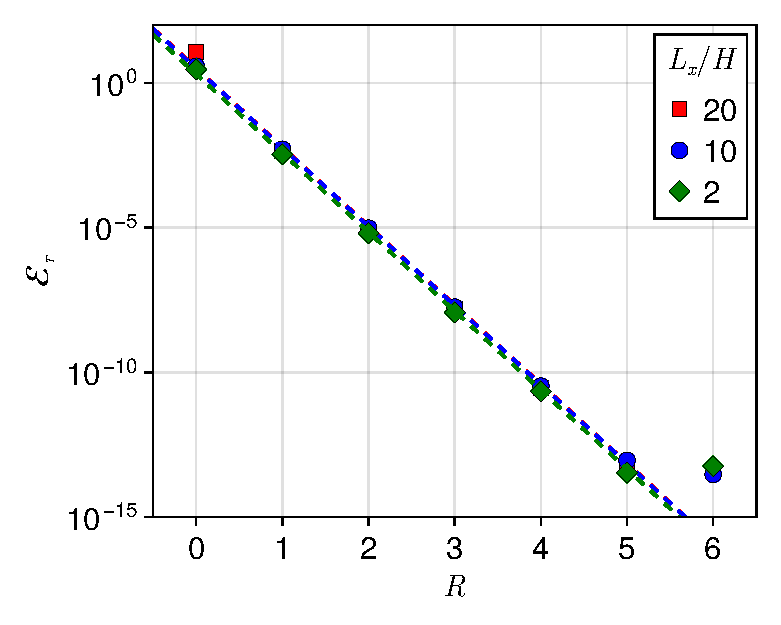
\includegraphics[width=0.55\linewidth]{figs/elc_error_force.pdf}
    \caption{Relative errors in force ($\mathcal{E}_r$) as a function of the padding ratio $R$ for systems without dielectric interfaces. 
    We consider systems with heights $H = 0.5, 1, 5$ while fixing $L_x=L_y=10$. The padding ratio is defined as $R = (L_z - H) / L_x$. The dashed lines represent the fitted curves with decay rates using theoretical prediction Eq.~\eqref{eq::ForceError}. }
    \label{fig:elc_error_force}
\end{figure}

Next, we examine systems with dielectric interfaces.
We set $\gamma_{\T u}=\gamma_{\T d}=\gamma$ and explore two prototypical scenarios by choosing $\gamma = 0.6$ and $1$, respectively. 
In both scenarios, the size of simulation box is fixed as $L_x=L_y=10$ and $H = 0.5$, and we vary the padding ratio $R$ (by changing $L_z$) and the image series truncation parameter $M$ to validate our theoretical results.
We first address the scenario with $\gamma = 0.6$, where we have $|g_{\T u}g_{\T d}| < 1$, so that the numerical errors are mainly contributed by the image series truncation error Eq.~\eqref{eq::Ferr1} and the ELC term Eq.~\eqref{eq::lhs_less1}.
% \begin{equation}\label{eq::0.6}
%     |\bm{F}_{\text{err}}^{M,i}| \sim \max \left\{ \lfloor(M+1)/2\rfloor^{-1}\left|\gamma_{\T u}\gamma_{\T d}\right|^{\lfloor\frac{M+1}{2}\rfloor} e^{-\frac{4\pi H\lfloor (M+1)/2\rfloor}{\max\{L_x,L_y\}}}, ~(g_{\T u}+g_{\T d}+2)e^{-\frac{2\pi L_z}{\max\{L_x,L_y\}}} \right\}\;.
% \end{equation}
The numerical results, as shown in Fig.~\ref{fig:error_icm_pad_gamma_0.6_force}, demonstrate that the errors in force decay exponentially with both the padding ratio $R$ and the number of image charge layers $M$, consistent with our theoretical predictions. Notice that in Fig.~\ref{fig:error_icm_pad_gamma_0.6_force} (a), the errors saturate at certain accuracy levels, this is due to the fixed image series truncation error (as we fix $M$). Similarly, the errors saturate in Fig.~\ref{fig:error_icm_pad_gamma_0.6_force} (b) as they reach the fixed ELC errors for given padding ratios $R$.
\begin{figure}[htbp]
    \centering
    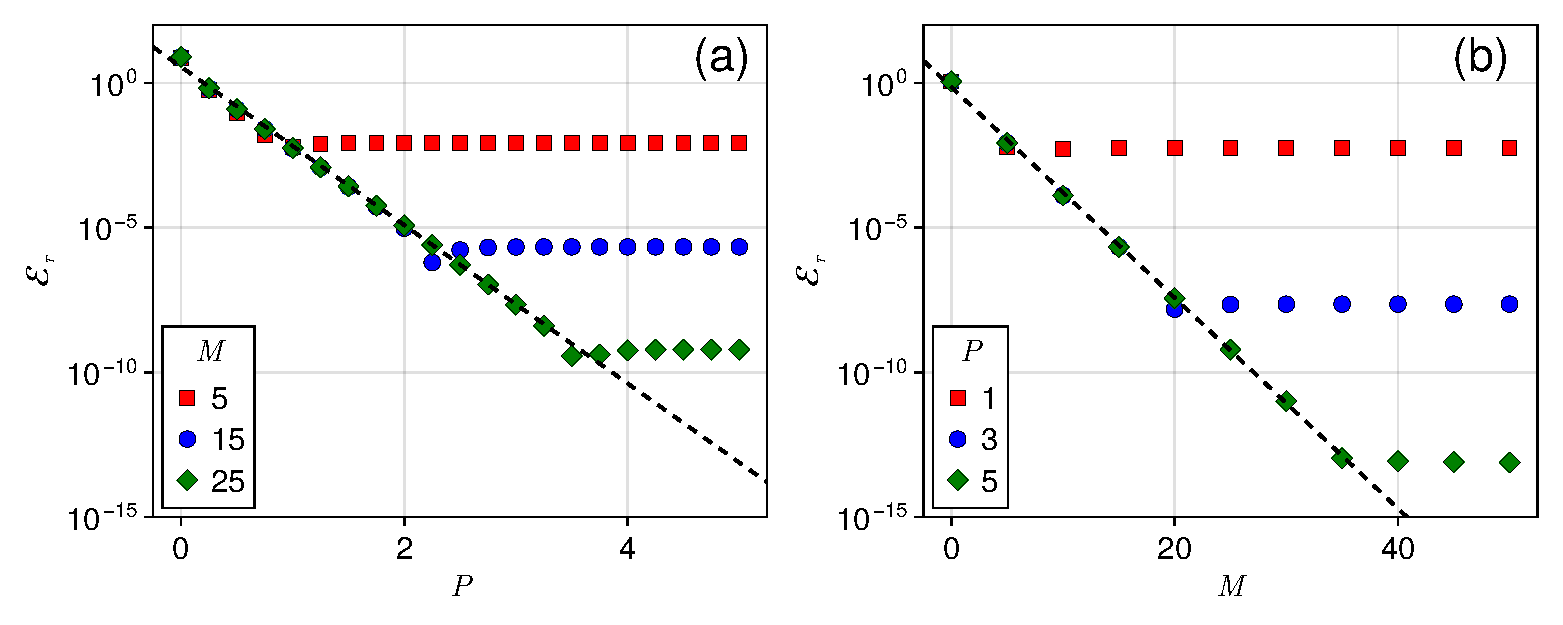
\includegraphics[width=0.98\linewidth]{figs/error_icm_pad_gamma_0.6_force.pdf}
    \caption{Relative errors in force ($\mathcal{E}_r$) for systems with dielectric interfaces. Here we fix $\gamma_{\T u}=\gamma_{\T d}=\gamma = 0.6$, $L_x=L_y=10$ and $H = 0.5$. 
    Panel (a) illustrates errors as a function of padding ratio $R$ with fixed image charge layers ($M=5,~15,~25$); panel (b) illustrates errors as a function of $M$ with fixed padding ratios ($R = 1,~3,~5$). The dashed lines in (a) and (b) represent the fitted curves with decay rates using theoretical predictions Eq.~\eqref{eq::lhs_less1} and Eq.~\eqref{eq::Ferr1}, respectively.}
    \label{fig:error_icm_pad_gamma_0.6_force}
\end{figure}

Now consider the scenario with $\gamma = 1$, where we have $|g_{\T u}g_{\T d}| > 1$, so that the numerical errors associated with the ELC term are described by Eq.~\eqref{eq::lhs_bigger1}.
In this context, the error behavior becomes more complex: as $M$ increases, the ELC error exhibits exponential growth, whereas the image truncation error decreases exponentially.
As illustrated in Fig.~\ref{fig:error_icm_pad_gamma_1_force} (a), by fixing $M$, we still observe exponential convergence in forces as the padding ratio $R$ increases. 
However, for a fixed padding ratio $R$, the errors display non-monotonic behavior with increasing $M$, as depicted in Fig.~\ref{fig:error_icm_pad_gamma_1_force} (b).
This subtle phenomenon was not fully understood since its first observation in the work of Yuan \emph{et al.}~\cite{yuan2021particle}. 
Our analysis reveals it as the combined effect of image truncation and ELC errors: 
initially, errors decrease due to the decay of image truncation errors; and once $M$ surpasses a certain $P$-dependent threshold, the error amplification mechanism predicted by Eq.~\eqref{eq::lhs_bigger1} becomes dominant, causing errors to grow exponentially.
Finally, we note that in strongly-confined systems, the presence of dielectric interfaces would introduce additional computational challenges~\cite{dos2015electrolytes}. 
Specifically, for systems with higher aspect ratios, a larger $M$ is required to achieve the same level of accuracy. The relevant numerical results are summarized in Section 2 of the SI. 
\begin{figure}[htbp]
    \centering
    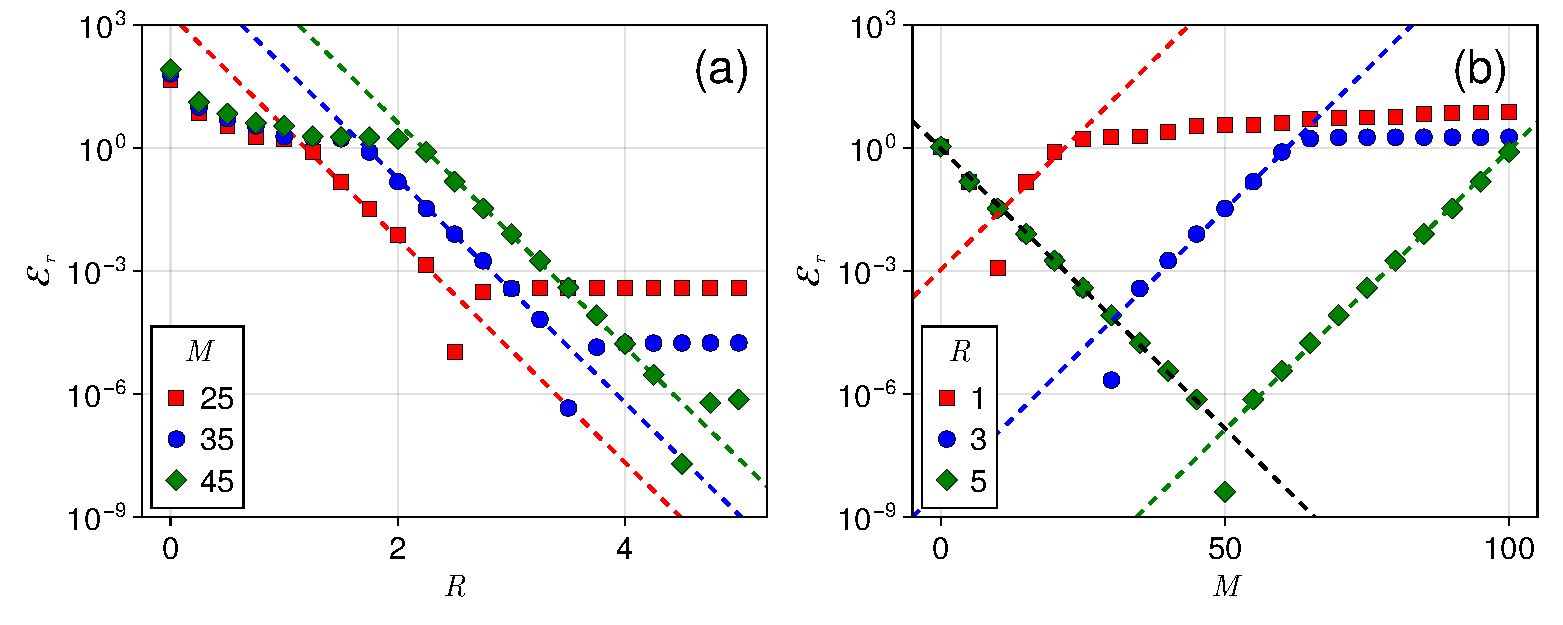
\includegraphics[width=0.98\linewidth]{figs/error_icm_pad_gamma_1_force.pdf}
    \caption{Relative errors in force ($\mathcal{E}_r$) for systems with dielectric interfaces. Here we fix $\gamma_{\T u}=\gamma_{\T d}=\gamma = 1$, $L_x=L_y=10$ and $H = 0.5$. 
    Panel (a) illustrates errors as a function of padding ratio $R$ with fixed image charge layers ($M=25,~35,~45$); panel (b) illustrates errors as a function of $M$ with fixed padding ratios ($R = 1,~3,~5$). The dashed lines in (a) and (b) represent the fitted curves with decay/growth rates using theoretical predictions Eq.~\eqref{eq::lhs_bigger1} and Eq.~\eqref{eq::Ferr1}.}
    \label{fig:error_icm_pad_gamma_1_force}
\end{figure}

% In practical simulations, especially when studying thin membranes, carbon nanotubes, and supercapacitors, accurately capturing the effects of nanoconfinement, i.e., when $H \ll \max\{L_x,L_y\}$, is crucial. Previous works have numerically shown that more image layers are needed to achieve satisfactory accuracy~\cite{dos2015electrolytes}. To further investigate the behavior of strongly confined systems, we present the error in force in \Cref{fig:icm_elc_error_force}, where we set $L_x=L_y=10$, $(L_z-H)/L_x = 5$ and consider system heights $H = 0.5, 1, 5$ while varying the number of image charge layers $M$. In \Cref{fig:icm_elc_error_force} (a), for $\gamma = 0.6$, we observe that the error decays exponentially as $M$ increases for $H = 0.5$ and $H = 1$. However, for $H = 5$, where $\gamma e^{2\pi H / L_x} > 1$, the error initially decreases before increasing as $M$ rises. This behavior is consistent with our theoretical predictions in Eqs.~\eqref{eq::FerrM} and \eqref{eq::FerrModd}. In \Cref{fig:icm_elc_error_force} (b), with $\gamma = 1$, we observe a similar pattern, where the error first decreases and then increases with increasing $M$. Furthermore, we note that the rate of increase depends on the aspect ratio $H/L_x$. A higher aspect ratio leads to a faster increase or decrease in error as $M$ is less or greater than the critical value that minimizes the error, respectively. This is also in alignment with our theoretical results in Eqs.~\eqref{eq::FerrM} and \eqref{eq::FerrModd}.

% \begin{figure}[htbp]
%     \centering
%     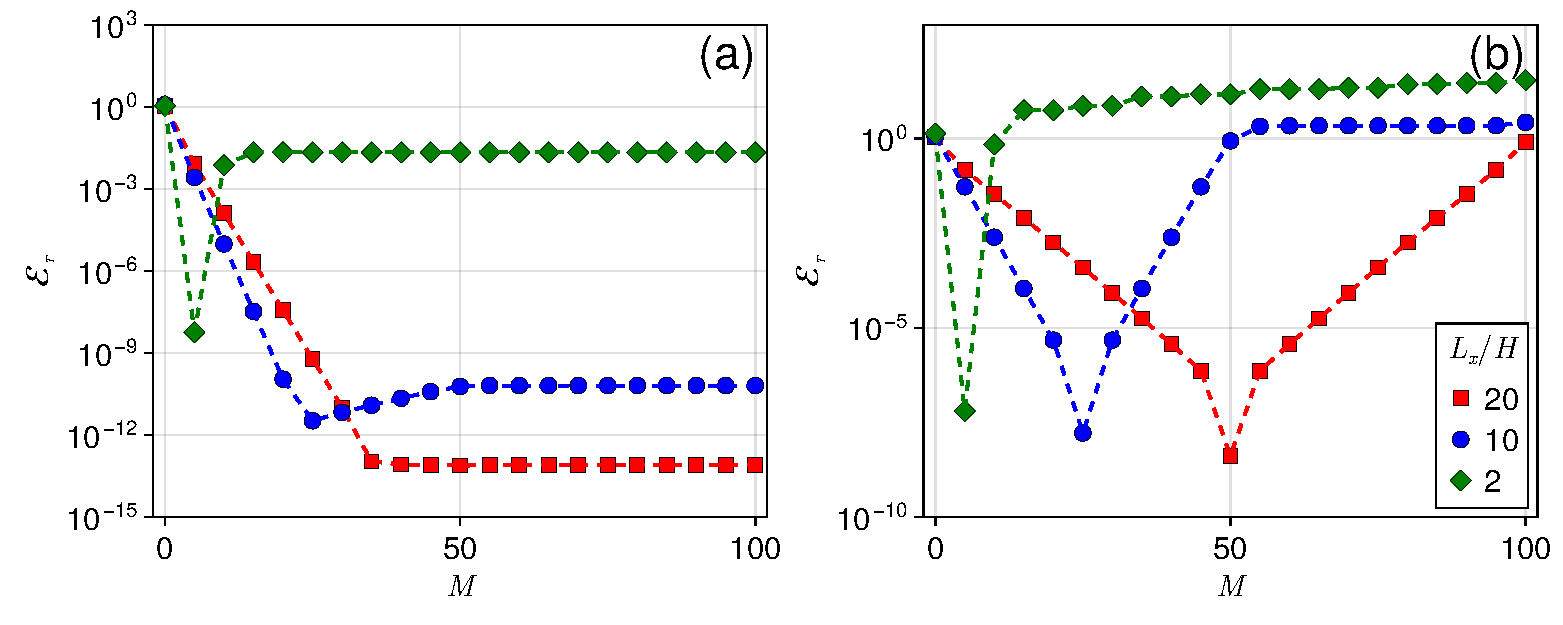
\includegraphics[width=0.98\linewidth]{figs/icm_elc_error_force.pdf}
%     \caption{Relative error of force ($\mathcal{E}_r$) in a dielectric-confined Coulomb system with parameters $P = 5$ and $H = 0.5, 1, 5$. In panels (a) and (b), the dielectric contrasts are set to $\gamma_{\T u} = \gamma_{\T d} = \gamma = 0.6$ and $\gamma_{\T u} = \gamma_{\T d} = \gamma = 1$, respectively.}
%     \label{fig:icm_elc_error_force}
% \end{figure}

As a final example, we validate our theoretical findings by replicating the non-monotonic error behavior reported by Yuan \emph{et al.} in figure 2 of Ref~\cite{yuan2021particle}. 
The reproduced numerical results are shown in Fig.~\ref{fig:error_yuan}, where we examine systems of dielectric-confined 2:1 electrolytes with $L_x = L_y = 15$ and $H = 5$. 
The three panels in Fig.~\ref{fig:error_yuan} correspond to systems with different reflection factors: $\gamma_{\T u} = \gamma_{\T d} = \gamma = 0.6$, $0.95$, and $1$, respectively. 
Within each panel, $L_z$ is varied as $45$, $75$, and $105$.
Note that for all cases considered here, the condition $|g_{\T u}g_{\T d}| > 1$ is satisfied, suggesting a similar phenomenon to that shown in Fig.~\ref{fig:error_icm_pad_gamma_1_force} (b), where errors diverge exponentially as $M$ surpasses a certain threshold.
Finally, we fit the numerical results using an analytical expression that combines the two primary error terms, Eq.~\eqref{eq:Uerr} and Eq.~\eqref{eq::U_ELC}, with coefficients determined through fitting.
The fitted curves, represented by dashed lines in Fig.~\ref{fig:error_yuan}, exhibit excellent agreement with the numerical data, thereby validating our theoretical predictions.

\begin{figure}[htbp]
\centering
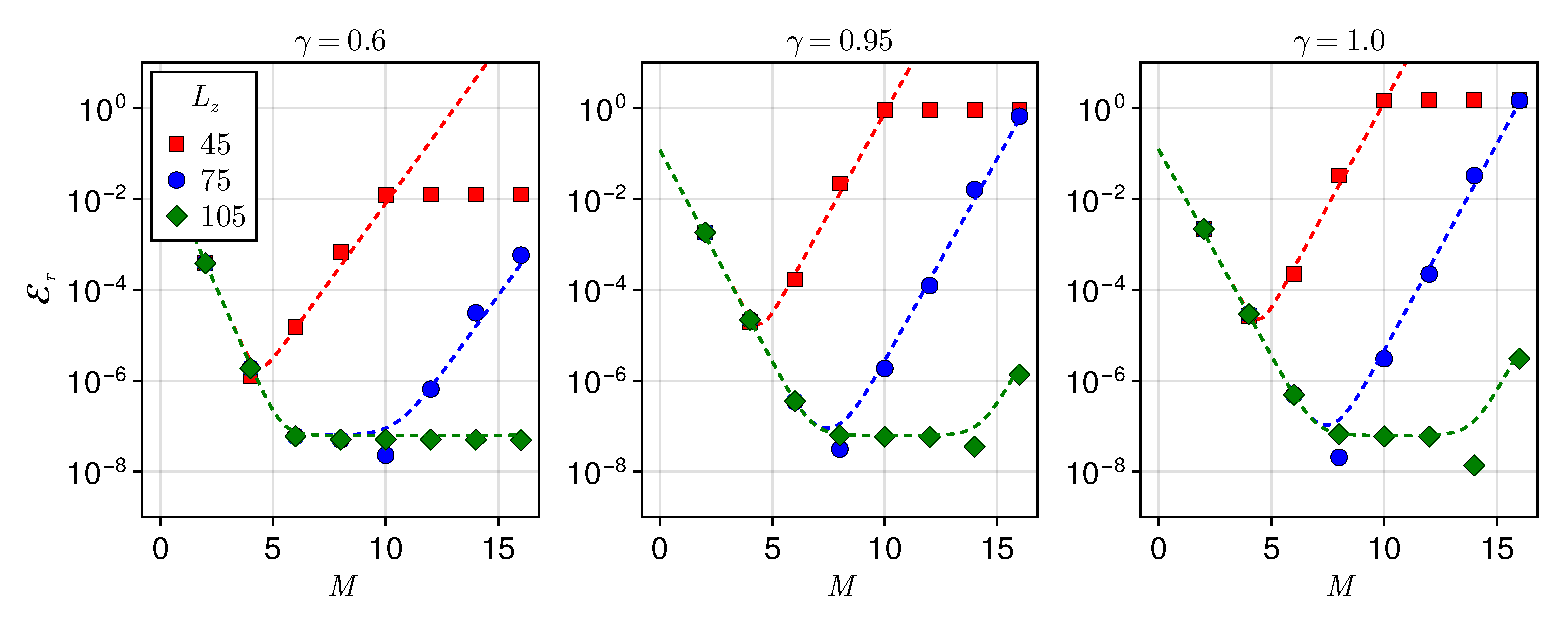
\includegraphics[width=0.98\linewidth]{figs/error_yuan.pdf}
\caption{
Relative errors ($\mathcal{E}_r$) in electrostatic energy for systems of 2:1 electrolytes with dieletric interfaces. 
Here we consider the same system setup studied by Yuan \emph{et al.}~\cite{yuan2021particle} using the ICM-PPPM method with $\gamma_{\T u}=\gamma_{\T d}=\gamma$ = 0.6, 0.95, and 1 (from left to right), respectively. In each panel, we fix $L_x = L_y = 15$, $H = 5$, and consider $L_z=$$45$, $75$, and $105$. 
Finally, the dashed lines represent the fitted curves using the sum of Eqs.~\eqref{eq:Uerr} and~\eqref{eq::U_ELC} (with coefficients determined by fitting).
}
\label{fig:error_yuan}
\end{figure}

\subsection{Optimal parameter selection strategy}\label{sec:parameter}
In practical simulations of dielectric-confined systems, a systematic strategy for determining the optimal algorithm parameters is highly beneficial. Specifically, given a prescribed error tolerance $\varepsilon$, it is crucial to identify parameter choices that achieve this tolerance with minimum computational cost. 
For ICM-Ewald3D~\cite{dos2015electrolytes} and ICM-PPPM~\cite{yuan2021particle} algorithms, 
our error analysis indicates that four interrelated parameters must be determined to control accuracy: 1). the Ewald splitting parameter $\alpha$, 2). the real-space cutoff $r_c$, 3). the image charge series truncation parameter $M$, and 4). the padding length $L_z$. 
By combining the error estimates from this study with the established Ewald splitting error, the overall error estimates for the ICM-Ewald3D and ICM-PPPM methods can be expressed as follows:
\begin{equation}\label{eq:error_icmelc}
\resizebox{0.8\width}{!}{\(
%|U_{\T{err}}|\sim|\bm{F}_{\T{err}}^{i}| 
\varepsilon \sim O\left(\frac{e^{-s^2}}{s^2}+\abs{\gamma_{\T u} \gamma_{\T d}}^{\lfloor\frac{M+1}{2}\rfloor} e^{-\frac{4\pi H \lfloor\frac{(M+1)}{2}\rfloor}{\max\{L_x,L_y\}}} + e^{-\frac{2\pi(L_z-H)}{\max\{L_x,L_y\}}} + \sum\limits_{l=1}^{M}C_{\gamma}^{(l)}e^{-\frac{2\pi(L_z-(l+1)H)}{\max\{L_x,L_y\}}}+e^{-\alpha^2 (L_z-H)^2}\right)\;,
\)}
\end{equation}
where the first term represents the Ewald decomposition error, the second term denotes the image charge series truncation error, the third and fourth terms correspond to the errors associated with the ELC term with image charges, and the last term corresponds to the trapezoidal discretization error.
Recall that, based on our analysis, the fourth term can grow exponentially with increasing $M$ if the condition $|g_{\T u}g_{\T d}| > 1$ is met. 
As a result, one should be careful in properly selecting the parameter $M$. 
Choosing a very large $M$ will not only increase the computational cost, but may also lead to incorrect results under certain circumstances.
In what follows, we propose an optimal parameter selection strategy based on the theoretical guidance of Eq.~\eqref{eq:error_icmelc}.

\emph{Step 1}: select $M$, so that the second term in Eq.~\eqref{eq:error_icmelc} is controlled by $\varepsilon$. 
There are three possible cases depending on the system setups:
\begin{enumerate}
    \item \textbf{Case 1}: If there is no dielectric interface, i.e., $\gamma_{\T u}=\gamma_{\T d}=0$, one simply set $M=0$.
    \item \textbf{Case 2}: If there is only one dielectric interface, i.e., either $\gamma_{\T u}=0$,$~\gamma_{\T d}\neq 0$ or $\gamma_{\T u}\neq 0$,$~\gamma_{\T d}=0$, one can set $M=1$ (since there is no image charge reflection).
    \item \textbf{Case 3}: If there are two polarizable dielectric interfaces, i.e., $\gamma_{\T u}\gamma_{\T d}\neq 0$, we select $M$ according to the following condition (obtained by algebraic manipulations of Eq.~\eqref{eq:Uerr}):
    \begin{equation}\label{eq::38}
    M\sim \frac{2\log \varepsilon - \frac{4\pi H}{\max\{L_x,L_y\}} - \log|\gamma_{\T u} \gamma_{\T d}|}{\log|\gamma_{\T u} \gamma_{\T d}| - \frac{4\pi H}{\max\{L_x,L_y\}}}\;.
\end{equation}
\end{enumerate}

\emph{Step 2}: select $L_z$, such that the sum of the third and fourth terms in Eq.~\eqref{eq:error_icmelc} is controlled by $\varepsilon$. 
Based on the leading-order error analysis presented in Section~\ref{sec::leadingerr}, two cases should be considered: 
\begin{enumerate}
    \item \textbf{Case 1}: If the condition $|g_{\T u}g_{\T d}|=\left|\gamma_{\T u}\gamma_{\T d}e^{\frac{4\pi H}{\max\{L_x,L_y\}}}\right|<1$
is satisfied, we have
\begin{equation}\label{eq::Lz_gamma_u_gamma_d_less1}
    L_z \geq H + \frac{\max\{L_x,L_y\}}{2\pi} \left( \log\frac{1}{\varepsilon} + \log \abs{\gamma_{\T u} + \gamma_{\T d} + e^{- \frac{2\pi H}{\max\{L_x,L_y\}}}} \right)\;.
\end{equation}
Note that for this case, $L_z$ can be chosen independent of $M$.
\item \textbf{Case 2}: If $\left|\gamma_{\T u}\gamma_{\T d}e^{\frac{4\pi H}{\max\{L_x,L_y\}}}\right|\geq 1$, we obtain
\begin{equation}\label{eq::Lz_gamma_u_gamma_d_greater1}
    L_z \geq (M + 1) H + \frac{\max\{L_x,L_y\}}{2\pi} \left( \log\frac{1}{\varepsilon} + \log \abs{\gamma_{\T u} \gamma_{\T d}} \right)\;.
\end{equation}
\end{enumerate}
It is interesting to note that, the selection of $L_z$ as derived in Eq.~\eqref{eq::Lz_gamma_u_gamma_d_greater1} can be interpreted physically as ensuring a sufficiently large vacuum layer in $z$ such that all the image charges can not overlap each other due to the periodic boundary conditions (necessitating $L_z\geq (M+1)H$). Additionally, an extra buffer zone is required, the length of which is determined by the specific tolerance $\varepsilon$.

\emph{Step 3}. After $M$ and $L_z$ are determined, the Ewald splitting parameter $\alpha$ and real-space cutoff $r_c$ can be selected. 
As indicated by Eq.~\eqref{eq:error_icmelc}, the Ewald decomposition error is independent of both the image truncation and the ELC error terms. 
The only extra constraint comes from the trapezoidal discretization error, which is typically minor due to its rapid decay with increasing $L_z$.
Consequently, the standard strategy can be employed to choose these parameters by setting $\varepsilon = e^{-s^2}/s^2$ and solving for $s$, where $s=r_c/\alpha$. 
The specific values of $r_c$ and $\alpha$ can then be adjusted to balance the computational costs between real-space and reciprocal-space calculations~\cite{frenkel2023understanding}.
Finally, to guarantee that the trapezoidal discretization error has been controlled, it is necessary to verify that the following condition is satisfied: 
\begin{equation}
    \alpha \geq (L_z-H)^{-1}\sqrt{\log\varepsilon^{-1}}\;.
\end{equation}
If this condition is not met, then $\alpha$ must be relaxed to fulfill this constraint.

We finally validate the proposed parameter selection strategy through numerical tests on two prototypical dielectric-confined systems, characterized by $\gamma_{\T u} = \gamma_{\T d} = 0.6$ and 1, respectively. 
The system dimensions are fixed at $L_x=L_y=10$ and $H = 1$. 
Note that for the system with $\gamma=0.6$, we have $|g_{\T u}g_{\T d}|<1$, while for the system with $\gamma=1$, $|g_{\T u}g_{\T d}|>1$.
For each system, the error tolerance $\varepsilon$ is set to $\epsilon = 10^{-4}$, $10^{-8}$, and $10^{-12}$. 
By applying the parameter selection strategy discussed earlier, we are able to select the optimized parameters and the results are summarized in Fig.~\ref{tab:parameter_selection_results}. 
Detailed error curves as functions of $M$ and $L_z$ are plotted in Fig.~\ref{fig:error_parameter_selection_force}, where the solid markers denote the specific parameter chosen via the proposed strategy.
\begin{table}[htbp]
    \centering
    \begin{tabular}{|c|c|c|c|c|}
        \hline
        $\gamma$ & $\epsilon$ & $s$ & $M$ & $L_z$ \\
        \hline
        $0.6$ & $10^{-4}$ & 3 & 9 & 15 \\
        $0.6$ & $10^{-8}$ & 4 & 17 & 30 \\
        $0.6$ & $10^{-12}$ & 5 & 25 & 45 \\
        $1$ & $10^{-4}$ & 3 & 16 & 32 \\
        $1$ & $10^{-8}$ & 4 & 31 & 62 \\
        $1$ & $10^{-12}$ & 5 & 45 & 91 \\
        \hline
    \end{tabular}
    \caption{Algorithm parameters $s$,~$M$ and $L_z$ for varied tolerance $\epsilon = 10^{-4}$, $10^{-8}$, and $10^{-12}$. 
    The parameters are selected according to the strategy proposed in this work. Two prototypical dielectric-confined systems are considered, with $\gamma=0.6$ and 1, respectively. Both systems have dimensions $L_x=L_y=10$ and $H = 1$.} \label{tab:parameter_selection_results}
\end{table}
\begin{figure}[!htbp]
    \centering
    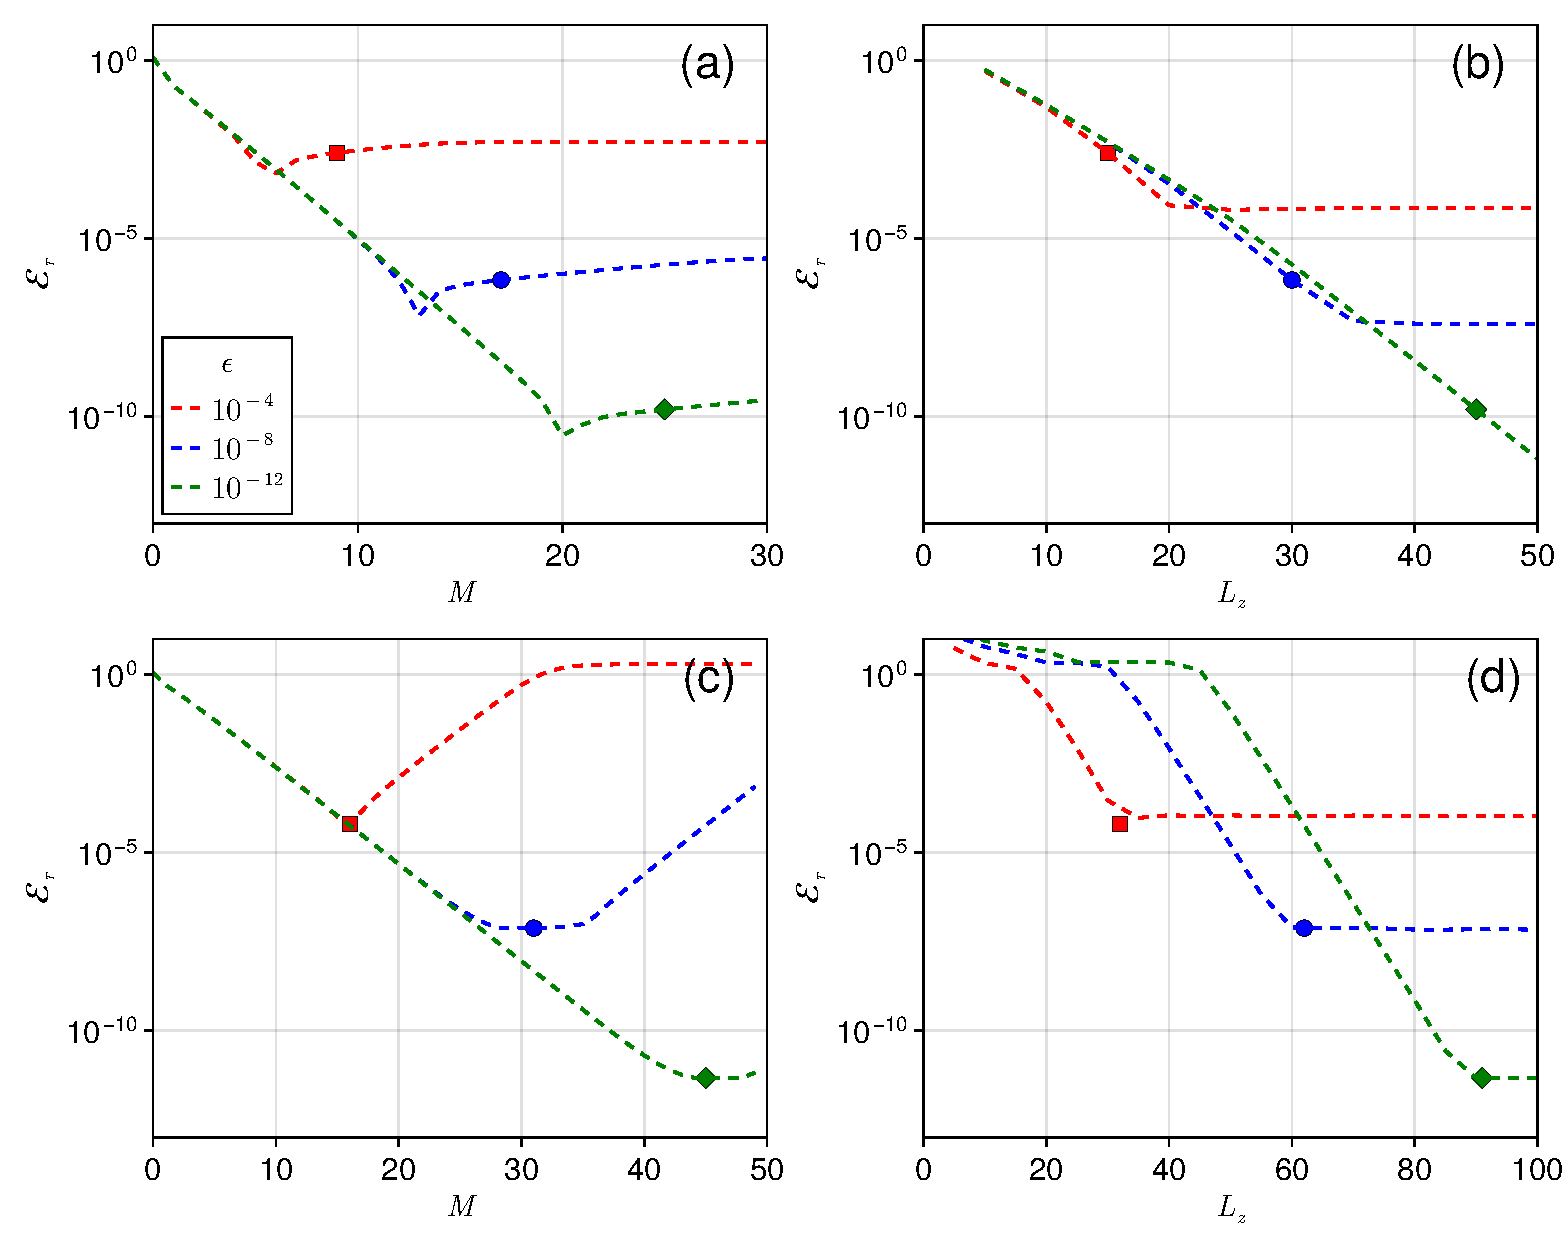
\includegraphics[width=0.92\linewidth]{figs/error_parameter_selection_force.pdf}
    \caption{
        Relative errors in force ($\mathcal{E}_r$) for two prototypical dielectric-confined systems with $\gamma=0.6$ (panels (a-b)) and $\gamma = 1$ (panels (c-d)), respectively.
        For both systems, we fix $L_x=L_y=10$ and $H = 1$. 
        Within each panel, the dashed lines correspond to the numerical errors obtained according to tolerance values $\epsilon = 10^{-4}$, $10^{-8}$, and $10^{-12}$, and the solid markers indicate the specific choice of $M$ or $L_z$ selected via the proposed strategy.
        Note that in panels (a) and (c), $s$ and $L_z$ are fixed according to Fig.~\ref{tab:parameter_selection_results}, whereas in panels (b) and (d), we fix $s$ and $M$.
    }
    \label{fig:error_parameter_selection_force}
\end{figure}
It is evident from Fig.~\ref{fig:error_parameter_selection_force} that, across all test cases with varying $\gamma$ and $\varepsilon$, the selected parameters consistently achieve optimal or near-optimal performance, especially for the case $\gamma = 1$. 
Consequently, we conclude that the parameter selection strategy proposed herein offers practical guidance for optimizing the performance of MD simulations of dielectric-confined systems.

\section{Random batch Ewald2D method}\label{sec::RBE2D}

In this section, we introduce the random batch Ewald2D (RBE2D) method, which is a mesh-free fast algorithm for computing the electrostatic force in quasi-2D systems.
After reformulating the Ewald2D summation as a 3D one, we can directly apply the RBE method to accelerate the reciprocal-space sum and reaching an optimal $O(N)$ scaling.
The detailed algorithm is presented in Subsection~\ref{subsec::RBE2D_algorithm}.
We then prove the unbiasedness and variance of the RBE2D method in Subsection~\ref{subsec::convergence}.
Finally, we extend the RBE2D method to dielectric-confined systems in Subsection~\ref{subsec::IBCELCDielectric}.

\subsection{The algorithm}\label{subsec::RBE2D_algorithm}

As been introduced in Section~\ref{sec::icm_ewald2d}, the Ewald2D summation can be reformulated as a 3D one, and here we apply the RBE method to accelerate the reciprocal-space sum.
Instead of deterministically computing the $\V k$-space sum in Eq.~\eqref{eq::U3D_Four} either directly or via FFT, we now evaluate it through a stochastic approximation, namely, the random ``mini-batch'' sampling~\cite{jin2020random}. 
Notice that the low $\V k$ modes are more important due to the $e^{-k^2/(4\alpha^2)}$ factor, an importance sampling strategy was further developed for variance reduction.
% The random batch Ewald (RBE) method has recently been developed for fully periodic systems~\cite{jin2021random,liang2022superscalability, liang2023random}, and here we extend it to quasi-2D systems.

The long-range component of the electrostatic force exerts on $i$-th particle is given by $\V F_i^{\ell}=-\nabla_{\bm{r}_i}U_{\ell}$, its random batch approximation is denoted as
\begin{equation}\label{eq:forceRBE}
\begin{aligned}
    \V {\tilde{F}}_i^{\ell}=-\sum_{\eta=1}^P \frac{S}{P}\frac{4\pi q_i\V k_\eta}{Vk_\ell^2} \te{Im}\left(e^{-\i \V k_\eta\cdot \V r_i}\rho(\V k_\eta)\right)\;,
\end{aligned}
\end{equation}
where $P$ is the batch size, $V=L_xL_yL_z$ is the volume of the extended simulation domain $\Omega_{\text{3D}}$, 
 {
$\rho(\V{k})$ is the \textit{structure factor} defined as
\begin{equation}
    \rho(\V{k})=\sum_{j=1}^N q_j e^{\i \V k\cdot \V r_j}\;,
\end{equation}
}
and $S$ is the normalizing constant,
\begin{equation}\label{eq:normalizingS}
\begin{aligned}
S=\sum_{\V k \neq 0} e^{-k^2/(4\alpha^2)}\;.
\end{aligned}
\end{equation}
%Due to the high-dimensional separability of the Gaussian function, 
In MD simulations, it is convenient to employ the Metropolis algorithm~\cite{metropolis1953equation} to sample from $\mathscr{P}(\bm{k})=e^{-k^2/(4\alpha^2)}/S$. 
 {Our numerical experiments indicate that the average acceptance rate exceeds $90\%$, rendering the correlation between samples negligible. In practice, one can further introduce a downsampling factor $\mathcal{P}$, namely, select $1$ sample from every $\mathcal{P}$ sampling steps to further eliminate the correlation (we take $\mathcal{P}=5$ in our calculations, and the autocorrelation decays to approximately $10^{-3}$, which is already a very small value), and this downsampling factor does not compromise overall efficiency, as the cost of sampling procedure is relatively low. Note that alternative methods, such as directly sampling from discrete multivariate Gaussian distributions by truncating at certain $k_{\mathrm{max}}$, are also applicable.}

%It should be noted that, the Metropolis algorithm generated samples are auto-correlated, to further reduce the variance, we take $1$ sample out of every $5$ sampling steps, to ensure successive samples are uncorrelated.}
% {Additionally, the acceptance rate is very high (more than $80\%$), so that the computational cost for sampling is negligible.}
%rev{An alternative, and presumably more efficient sampling approach is to directly sample from $\mathscr{P}(\bm{k})$, which requires truncating the series summation~Eq.~\eqref{eq:normalizingS} at certain $k_{\mathrm{max}}$.}

For quasi-2D systems, the RBE2D method offers a particular advantage: it is mesh free, so that unlike existing grid-based fast algorithms, the computational cost is independent   {of the} added vacuum layer thickness. This statement is justified more rigorously in Theorem~\ref{Thm::1}. 
 {In the theorem, one utilizes the Debye-H\"uckel (DH) assumption for non-ideal electrolytes~\cite{levin2002electrostatic} (also see Appendix F in \cite{gan2024fast}), where the ensemble-averaged charge distributions around a charged particle follow the Boltzmann distribution.
}

\begin{thm}\label{Thm::1} 
    Denote the fluctuation of the random batch approximation in force by $\V \Xi_{\V F,i}=\V {\tilde{F}}_i^{\ell}-\V {F}_i^{\ell}$. The random variable $\V \Xi_{\V F,i}$ has zero expectation, i.e., $\mathbb{E}\V \Xi_{\V F,i}=\V 0$, and its variance is given by
    \begin{equation}\label{eq::30}
        \mathbb{E}|\V \Xi_{\V F,i}|^2=\frac{1}{P}\left[\frac{(4\pi q_i)^2S}{V^2}\sum_{\bm{k}\neq \bm{0}}\frac{e^{-k^2/(4\alpha^2)}}{k^2}\left|\emph{Im}\left(e^{-\i \V k \cdot \V r_i}\rho(\V k)\right)\right|^2-|\V F_{i}^{\ell}|^2\right]
    \end{equation}
    which is bounded and scales as $\mathcal O(1/P)$. Furthermore, under the DH assumption, $\mathbb{E}|\V \Xi_{\V F,i}|^2$ is independent of both the particle number $N$ and the size $L_z$.
\end{thm}

\begin{proof}%[Proof of \emph{Theorem}~\emph{\ref{Thm::1}}]
    The property of unbiasedness in Theorem~\ref{Thm::1} is straightforward and guarantees the consistency of the stochastic approximation, i.e., $\mathbb{E}\V{ \tilde{F}}_i^{\ell}=\mathbb{E}\V {F}_i^{\ell}$. 
    Let us now consider the variance.
    By the DH assumption, the structure factor term in Eq.~\eqref{eq::30} is bounded by a constant $C$~\cite{jin2021random} for $\bm{k}\neq \bm{0}$,
    \begin{equation}
        \left|\te{Im}\left(e^{-\i \V k\cdot \V r_i}\rho(\V k)\right)\right|^2\leq C,
    \end{equation}
    and vanishes for $\bm{k}=\bm{0}$. 
    Further by the monotonicity of Gaussian on $[0, +\infty )$, it follows that
    \begin{equation}\label{eq::32}
        \begin{split}
            \mathbb{E}|\V \Xi_{\V F,i}|^2\leq \frac{8 CSq_i^2}{PV}\int_{0}^{\infty}e^{-k^2/(4\alpha^2)}dk= \frac{8\sqrt{\pi}\alpha CSq_i^2}{PV}\;.%\mathbb{E}|\V \Xi_{\V F,i}|^2&\leq\frac{(4\pi q_i)^2CS}{PV^2}\sum_{\bm{k}\neq\bm{0}}\frac{e^{-k^2/(4\alpha^2)}}{k^2}\leq \frac{8 CSq_i^2}{PV}\int_{0}^{\infty}e^{-k^2/(4\alpha^2)}dk= \frac{8\sqrt{\pi}\alpha CSq_i^2}{PV}\;.
        \end{split}
    \end{equation}
    Analogously, one can obtain the following estimate for the normalization constant $S$:
    \begin{equation}\label{eq::Sa}
        \begin{split}
            S\leq \frac{V}{(2\pi)^3}\int_{0}^{\infty}4\pi k^2e^{-k^2/(4\alpha^2)}dk=\frac{\alpha^3V}{\pi^{3/2}}.
        \end{split}
    \end{equation}
    Substituting Eq.~\eqref{eq::Sa} into Eq.~\eqref{eq::32} yields
    \begin{equation}
        \mathbb{E}|\V \Xi_{\V F,i}|^2\leq\frac{8\alpha^4Cq_i^2}{\pi P}\sim \mathcal O\left(\frac{1}{P}\right)
    \end{equation}
    which is independent of either $N$ or $L_z$.
\end{proof}

Theorem~\ref{Thm::1} suggests that the variance in the random batch approximation can be effectively controlled %within the mean-field region 
by appropriately choosing the batch size $P$, which is independent   {of the} particle number $N$.
In the context of Ewald summation, typical choices for $\alpha$ are $(\sqrt{N}/V)^{1/3}$ for direct truncation~\cite{kolafa1992cutoff} and $(N/V)^{1/3}$ for FFT-based calculation~\cite{deserno1998mesh}. 
%For RBE2D, select $\alpha\sim \rho_{r}^{1/3}$, which ensures efficient real space computations and accelerated Fourier space computations. When the system becomes more dilute due to an increase in $L_z$ while keeping $N$ fixed, the upper bound of the variance decreases at a rate of $O(L_z^{-4/3})$. 
Now for the RBE2D method, it is clear that changing the vacuum layer thickness does not affect its efficiency. 
%However, the practical case may deviate from this ideal assumption due to the spatial anisotropy of the ion distribution, which is confined within the range of $[0,H]$. 
In practice, we set $\alpha\sim N^{1/3}/(L_xL_yH)^{1/3}$ (independent of $L_z$), then it is expected that the variance of the force remains at the same level as one changes $L_z$.
This is further validated by numerical results in Section~\ref{subsec::electrolyte-neutral}.

\subsection{Convergence and complexity of the RBE2D} \label{sec::convergence}

In this section, we further examine the convergence and complexity of RBE2D accelerated MD simulations. 
First, we revisit the the common purpose of MD simulations, which is to explore the configuration space and obtain static/dynamic ensemble-averaged properties by solving the equations of motion for $N$ interacting particles.
For example, consider the widely used canonical ensemble, where the system has fixed particle number $N$, volume $V$ and temperature $T$, which can be simulated as solving the following equations, namely, MD with Langevin thermostat~\cite{frenkel2023understanding}:
\begin{equation}\label{Langevin}
    \begin{aligned}
        & d \bm{r}_i=\bm{v}_i d t, \\
        & m_i d \bm{v}_i=\left[\bm{F}_i-\gamma \bm{v}_i\right] d t+\sqrt{2 \gamma k_{\mathrm{B}} T} d \bm{W}_i,
    \end{aligned}
\end{equation}
where $\bm{r}_i$, $m_i$, and $\bm{v}_i$ represent the position, mass, and velocity of the $i$-th particle, respectively. $\V{F}_i$ is the force exert {ed} on the $i$-th particle, $\{\bm{W}_i\}$ are i.i.d.~Wiener processes, and $\gamma$ is the reciprocal characteristic time scale associated with the thermostat.
In practice, the stochastic differential equations are discretized with proper numerical schemes and integrated with time step~$\Delta t$.
Let~$(\V{r}_i, \V{v}_i)$ be the solution to Eq.~\eqref{Langevin} with~$\bm{F}_i = \bm{F}^{\text{exact}}_i$, where~$\bm{F}^{\text{exact}}_i$ is the exact force on the $i$-th particle; and let $(\widetilde{\bm{r}}_i,\widetilde{\bm{v}}_i)$ be the solution to the same set of equations but with RBE2D approximated force given by~$\bm{F}_i = \bm{F}^{\text{exact}}_i + \bm{\Xi}_{\bm{F},i}$.
Then the relation between the two sets of solutions satisfies the following Theorem~\ref{thm::2}~\cite{jin2021convergence}.

\begin{thm}\label{thm::2}
If the forces $\bm{F}_i$ are bounded and Lipschitz, and the fluctuation of stochastic force satisfies $\mathbb{E}\V \Xi_{\V F,i}=0$, then for any $t_{\emph{MD}}>0$, there exists $C(t_{\emph{MD}})>0$ such that
\begin{equation}\label{eq::Convergence}
\sup _{t \in[0, t_{\emph{MD}}]} \sqrt{\frac{1}{N} \sum_{i=1}^N \mathbb{E}\left(\left|\bm{r}_i-\widetilde{\bm{r}}_i\right|^2+\left|\bm{v}_i-\widetilde{\bm{v}}_i\right|^2\right)} \leq C(t_{\emph{MD}}) \sqrt{\Lambda \Delta t}. %\sim C(t_{\emph{MD}}) \sqrt{\frac{\Delta t}{P}}.
\end{equation}
 {Here, $\Lambda$ is an upper bound for $\mathbb{E}|\V \Xi_{\V F,i}|^2$, and one has $\Lambda\sim \mathcal O(1/P)$ due to Theorem~\ref{Thm::1}.} 
\end{thm}

Theorem~\ref{thm::2} indicates that the RBE2D approximated dynamics is capable of capturing finite time structure and dynamic properties.
For long-time simulations, additional assumptions are needed regarding force regularity~\cite{jin2022random}. 
It   {is worth} noting that, although the Coulomb potential is neither bounded nor Lipschitz at $r=0$, actual MD simulations will include the Lennard-Jones (LJ) potential, which provides a  {strong repulsive force at short inter-particle distance and prevents the particles from getting too close. As a result, the singularities in both the Coulomb and LJ potentials will not be reached in practice as long as the time step is properly chosen, allowing to satisfy the condition of Theorem~\ref{thm::2}  for MD simulations.}

Additionally, following Theorem \ref{thm::2}, the fluctuations introduced by random batch approximation, $\V \Xi_{\V F,i}$,  can be physically understood as heating effects, which will cause a temperature drift for the system and is unwanted. 
For NVT and NPT ensembles, the heating effect can be eliminated by introducing appropriate thermostats such as the Langevin thermostat~\cite{feller1995constant}, the Nos\'e-Hoover (NH) thermostat~\cite{hoover1985canonical}, etc. With an additional weak-coupled bath on the Newtonian dynamics to avoid energy drift, the NVE ensemble can also be accurately simulated with random batch-type approximations~\cite{liang2024JCP}.

Next, we analyze the computational complexity of the RBE2D accelerated MD simulations. The detailed algorithm is summarized in Fig.~\ref{Alg::1}.  
In the RBE2D, the random batch importance sampling in Eq.~\eqref{eq:forceRBE} approximates the Fourier space force by summing over $P$ Fourier modes. 
At each step, $P$ structure factors, $\{\rho(\bm{k}_{\eta})\}_{\eta=1}^{P}$, are computed for all particles, resulting in a Fourier part complexity of $\mathcal{O}(PN)$. Furthermore, as shown in Theorems~\ref{Thm::1} and \ref{thm::2} and the analysis at the end of Section~\ref{subsec::RBE2D_algorithm}, the RBE2D error does not grow as $N$ or $L_z$ increases when the batch size $P=\mathcal{O}(1)$ and $\alpha\sim N^{1/3}/(L_xL_yH)^{1/3}$ are provided. 
The real space part of the RBE2D is short-ranged due to the rapid decay of factor $\erfc(\alpha r)$ and can be directly truncated by introducing a cutoff $r_c$. 
As a result, the real space complexity is proportional to the product of $N$ and the average number of neighbors within a volume of $4\pi r_c^3$ per particle. 
For a given truncation error tolerance, $r_c\sim \alpha^{-1}$, yielding a real space complexity $\sim \alpha^{-3}N/(L_xL_yH)=\mathcal{O}(1)$ per particle. 
As such, the total computational complexity is of $\mathcal{O}(N)$. 

\begin{algorithm}[ht]
 \caption{(RBE2D accelerated molecular dynamics for quasi-2D systems)}\label{Alg::1}
 \begin{algorithmic}[1]
  \State Choose $\alpha$, $r_c$ (the cutoff in real space), $\Delta t$, the vacuum layer parameter $L_z$, and batch size $P$. Initialize the positions and velocities of ions as well as surface charge densities. Set $N_T$ as the total MD time steps.
  \For {$n \text{ in } 1: N_T$}
  \State Sample $P$ nonzero frequencies $\bm{k}\sim e^{-k^2/(4\alpha)}$ by the Metropolis procedure to form  set $\mathcal{K}$.
  \State The $\V k$-space component of the force, $\bm{F}_i^{\ell}$, is computed using the random batch approximation $\widetilde{\V F}_i^{\ell}$ with the $P$ frequencies from the set $\mathcal{K}$.
  \State The real space component of the force, $\bm{F}_i^{s}$, is computed by the neighbor list method. %The rest force terms, including the YB correction $\V F_{i}^{\te{YB}}$, the renormalization term $\V F_{i}^{\te{renorm}}$, and the ion-wall force $\V F_{i}^{\te{wall}}$, can be directly computed.
  \State Integrate the equations of motion for time step $\Delta t$ with an appropriate thermostat and its corresponding integration scheme. %the total force
  %$$\V F_i=\widetilde{\V F}_i^{\ell}+\bm{F}_i^{\te{real}}+\V F_{i}^{\te{YB}} + \V F_{i}^{\te{wall}}$$
  
  \EndFor
 \end{algorithmic}
\end{algorithm}
Besides its linear complexity, the RBE2D method offers two other significant advantages:
\begin{itemize}
    \item  {Communication efficiency: The RBE2D method is embarrassingly parallel, requiring only a single global reduction of the structure factors for all $\mathcal{O}(P)$ samples when calculating the force using Eq.~\eqref{eq:forceRBE}.} This streamlined communication facilitates high scalability. 

    \item Vacuum layer flexibility: the RBE2D is mesh free, and choosing a larger vacuum layer thickness incurs no extra cost. This provides flexibility for one to always choose a proper $L_z$ to guarantee accuracy, without sacrificing efficiency.
\end{itemize}

\subsection{RBE2D method for dielectrically confined quasi-2D systems} \label{subsec::IBCELCDielectric}

We now extend the RBE2D method for efficient MD simulations of dielectrically confined quasi-2D Coulomb systems. 
First, given tolerance $\varepsilon$, one shall choose appropriate values for $M$ and $L_z$, such that the image series truncation error, the ELC term, and remainder error term can all be neglected. Then, let $\bm{F}_{\ell}^{\text{c}}$ denotes the $\V k$-space component of force acting on the $i$-th particle, it reads
\begin{equation}\label{eq::52}
\bm{F}_{\ell}^{\text{c}}(\bm{r}_i)=-\frac{2\pi}{L_xL_yL_z}\sum_{\bm{k}}{}^{\prime}\frac{e^{-\frac{k^2}{4\alpha^2}}}{k^2}\nabla_{\bm{r}_i}\left[\rho_{\bm{k}}\bar{\rho}_{\bm{k}}^{M}\right]+\bm{F}_{\text{IBC}}^{M}(\bm{r}_i)\;,%+\bm{F}_{\text{ELC}}^{M}(\bm{r}_i)+\bm{F}_{\text{err}}^{M}(\bm{r}_i)\;,
\end{equation}
where 
\begin{equation}\label{eq::rhorhoM}
\begin{split}
\nabla_{\bm{r}_i}\left[\rho_{\bm{k}}\bar{\rho}_{\bm{k}}^{M}\right]=&q_i\bm{k}\text{Im}\left[e^{-\i\bm{k}\cdot\bm{r}_i}\left(\rho_{\bm{k}}+\rho_{\bm{k}}^{M}\right)+\sum_{\substack{l=1\\ \text{even}}}^{M}\left(\gamma_{+}^{(l)}e^{-\i\bm{k}\cdot\bm{r}_{i+}^{(l)}}+\gamma_{-}^{(l)}e^{-\i\bm{k}\cdot\bm{r}_{i-}^{(l)}}\right)\rho_{\bm{k}}\right]\\
+&q_i\widehat{\bm{k}}\text{Im}\left[\sum_{\substack{l=1\\ \text{odd}}}^{M}\left(\gamma_{+}^{(l)}e^{-\i\bm{k}\cdot\bm{r}_{i+}^{(l)}}+\gamma_{-}^{(l)}e^{-\i\bm{k}\cdot\bm{r}_{i-}^{(l)}}\right)\rho_{\bm{k}}\right]
\end{split}
\end{equation}
with $\rho_{\bm{k}}^{M}$ the conjugate of $\bar{\rho}_{\bm{k}}^{M}$ and $\widehat{\bm{k}}=(k_x,k_y,-k_z)$. The calculation of Eq.~\eqref{eq::52} can also be accelerated via FFT, namely, the ICM-PPPM method~\cite{yuan2021particle}. 
If the image reflection level is truncated at $M$, the computational cost of ICM-PPPM is $\mathcal O(MN \log(MN))$. Thus for strongly confined systems, the cost of FFT-based method will increase rapidly as $M$ increases.
%This means that the cost does not increase rapidly as $M$ increases, which indicates that RBE2D is more suitable for systems with strong surface polarization. 
%The detailed formula is given in Eq.~\eqref{eq::F_c_Four_detail}.

We now again apply the importance sampling technique to approximate $\bm{F}_{\ell}^{\text{c}}$, yielding the following stochastic estimator as 
%More precisely, we regard the factor $e^{-\frac{k^{2}}{4\alpha^2}}$ as a discrete Gaussian distribution, and denote the resulting estimator of force as
\begin{equation}\label{eq::important}
\bm{F}_{\ell}^{\text{c}}(\bm{r}_i)\approx \bm{F}_{\ell}^{\text{c},*}(\bm{r}_i)=-\frac{2\pi }{L_xL_yL_z}\sum_{\eta=1}^{P}\frac{S}{P}\frac{\nabla_{\bm{r}_i}\left[\rho_{\bm{k}_{\eta}}\bar{\rho}_{\bm{k}_{\eta}}^{M}\right]}{k_{\ell}^2}+\bm{F}_{\text{IBC}}^{M}(\bm{r}_i),
\end{equation}
where $\{\bm{k}_{\eta}\}_{\eta=1}^{P}$ are the $P$ batches of wave vectors sampled from $\mathscr{P}(\bm{k})$. 
It is important to note that when surface charges are present at the interfaces~\cite{spohr1997effect,yi2017note,yuan2021particle}, a straightforward modification to Eq.~\eqref{eq::important} is required, which allows for the simultaneous treatment of discrete ions and continuous surface charges.
Detailed information can be found in the SM, Section S1.
And the real space component of force is given by Eq.~(SM1.3), which can still be evaluated by neighbor lists algorithms.

%The real space part of force, as given by Eq.~(SM1.3) in the SM, is computed via directly truncating at a cutoff radius $r_c$.
%In contrast to the fully periodic case, the choice of $r_c$ does not need to satisfy the minimum image principle along the $z$-direction. 
%For systems where $H\ll\min\{L_x,L_y\}$, selecting a larger $r_c$ can reduce the computational cost of the reciprocal space summation, but enlarges the number of included images as well, resulting in a decrease in efficiency.
%Hence, it is crucial to carefully calibrate $r_c$ with other parameters. 

Next, we describe a simple strategy for efficiently summing over the $2MN$ image charges.
% To reduce this cost, we present a more efficient approach. 
Notice that Eq.~\eqref{eq::rhorhoM} can be rewritten as
\begin{equation}\label{eq::56}
\begin{split}
    \nabla_{\bm{r}_i}\left[\rho_{\bm{k}}\bar{\rho}_{\bm{k}}^{M}\right]
    = & q_i\bm{k}\text{Im}\left[e^{-\i \bm{k}\cdot \bm{r}_i}\sum_{j=1}^{N}q_je^{\i\bm{k}\cdot\bm{r}_{j}}\left(1+e^{-2\i k_zz_j}Y_{\text{odd}}(k_z)+Y_{\text{even}}(k_z)\right)\right]\\
    + & q_i\bm{k}\text{Im}\left[e^{-\i \bm{k}\cdot\bm{r}_i}\left(1+e^{2\i k_zz_i}\overline{Y}_{\text{odd}}(k_z)\right)\rho_{\bm{k}}\right]+q_{i}\widehat{\bm{k}}\text{Im}\left[e^{-\i\bm{k}\cdot\bm{r}_i}\overline{Y}_{\text{even}}(k_z)\rho_{\bm{k}}\right],
\end{split}
\end{equation}
 {where the coefficients $Y_{\text{odd}}$ and $Y_{\text{even}}$ are defined as follows: 
\begin{equation}
    \begin{split}
        Y_{\text{odd}}(k_z) &= \sum_{\substack{l=1, \text{odd}}}^{M}\left[\gamma_{+}^{(l)}e^{\i k_z(l+1) H}+\gamma_{-}^{(l)}e^{-\i k_z (l-1)H}\right], \\ 
        Y_{\text{even}}(k_z) &= \sum_{\substack{l=1, \text{even}}}^{M}\left[\gamma_{+}^{(l)}e^{\i k_zl H}+\gamma_{-}^{(l)}e^{-\i k_z l H}\right].
    \end{split}
\end{equation}
This formulation enables the decoupling of the summation over particles index $j$ and their image index $l$. 
In practical simulations, one shall first precompute $Y_{\text{odd}}(k_z)$ and $Y_{\text{even}}(k_z)$ for each $\bm{k} \in \{\bm{k}_{\eta}\}_{\eta=1}^{P}$, as these are configuration independent, with a computational cost of $\mathcal{O}(PM)$. 
Subsequently, for a given particle configuration, one evaluates $\rho_{\bm{k}}$, along with the conjugates of $Y_{\text{odd}}$ and $Y_{\text{even}}$, and computes
\begin{equation}
    \sum_{j=1}^{N}q_je^{\i\bm{k}\cdot\bm{r}_{j}}\left(1+e^{-2\i k_zz_j}Y_{\text{odd}}(k_z)+Y_{\text{even}}(k_z)\right)
\end{equation}
for every $\bm{k}\in\{\bm{k}_{\eta}\}_{\eta=1}^{P}$, which incurs a cost of $\mathcal{O}(PN)$ operations. These intermediate variables are then utilized to evaluate $\nabla_{\bm{r}_i}\left[\rho_{\bm{k}}\bar{\rho}_{\bm{k}}^{M}\right]$ for all particles $i$ using Eq.~\eqref{eq::56}, adding another $\mathcal O(PN)$ to the cost. Finally, substituting the value of $\nabla_{\bm{r}_i}\left[\rho_{\bm{k}}\bar{\rho}_{\bm{k}}^{M}\right]$ into Eq.~\eqref{eq::important} allows for the computation of the first term on the right-hand side with $\mathcal{O}(PN)$ operations, followed by the addition of the IBC term, which incurs an $\mathcal{O}(N)$ cost. Consequently, the total computational cost for force evaluations is reduced from $\mathcal O(PMN)$ to $\mathcal O(P(M+N))$.
In practice, one shall still take $\alpha \sim N^{1/3}/(L_xL_yH)^{1/3}$ to ensure that the real space calculation costs $\mathcal{O}(N)$, then the $\V k$-space components of force can be calculated as such so that the complexity is reduced to $\mathcal{O}(P(M+N))$.}
Thus, the overall complexity of the RBE2D is approximately $\mathcal{O}(N)$ since both $P$ and $M$ are of $\mathcal O(1)$ and independent   {of} $N$.
The detailed algorithm for RBE2D accelerated MD in the presence of dielectric interfaces is summarized in Algorithm~\ref{alg::RBEalg}.

\begin{algorithm}[H]
 \caption{(RBE2D for quasi-2D systems under dielectric confinement)}\label{alg::RBEalg}
 \begin{algorithmic}[1]
  \State Choose $\alpha$, $r_c$ (the cutoff in real space), $\Delta t$, batch size $P$, image reflection level of truncation $M$, and the vacuum layer parameter $L_z$. Initialize the coefficients of dielectric jumps ($\varepsilon_{\rm{top}}$, $\varepsilon_{\rm{c}}$, $\varepsilon_{\rm{bot}}$) and the positions and velocities of charges $\bm{r}^0_i, \bm{v}^0_i$ for $1\le i\le N$. Set $N_T$ as the total MD time steps.
  %\State Sample sufficient number of nonzero $\bm{k}\sim e^{-k^2/(4\alpha)}$ by the MH procedure to form a set $\mathcal{K}$.
  \For {$n \text{ in } 1: N_T$}
  \State Sample $P$ nonzero frequencies $\bm{k}\sim e^{-k^2/(4\alpha)}$ by the Metropolis procedure to form set $\mathcal{K}$.
  \State The real space component of force is computed via a neighbor list algorithm (for both actual charges and image charges within $r_c$).
  \State The Fourier space component of  {the} force is computed via the random batch approximation $\bm{F}_{\ell}^{\text{c},*}$, with $P$ frequencies from the set $\mathcal{K}$.
  \State Integrate the equations of motions for time $\Delta t$ with  {an} appropriate integration scheme and some appropriate thermostat. 
  \EndFor
 \end{algorithmic}
\end{algorithm}

Finally, consider the fluctuation of random batch approximation of the force, denoted as $\bm{\Xi}_{\bm{F},i}^{\text{c}}=\bm{F}_{\ell}^{\text{c},*}(\bm{r}_i)-\bm{F}_{\ell}^{\text{c}}(\bm{r}_i)$, one can still show that 1) the variance of the RBE2D method is controlled via $\mathcal{O}(1/P)$ and is independent of $L_z$; 2) the RBE2D is capable to capture finite time structure and dynamic properties in MD simulations. 
The proof is similar to Theorems~\ref{Thm::1} and~\ref{thm::2}, and is thus omitted here.

\section{Numerical results on quasi-2D systems without dielectric interfaces}\label{sec::numerical}

In this section, numerical results are first presented for the homogeneous case, validating the performance of RBE2D accelerated MD simulations. 
Examples include coarse-grained model {s} of electrolytes and all-atom SPC/E bulk water systems~\cite{berendsen1987missing} confined by two slabs without dielectric jumps,  {where all the quantities are defined and calculated in reduced LJ units and real units~\cite{frenkel2023understanding}, respectively.}
Our method is implemented in LAMMPS (version 29Oct2020) \cite{thompson2021lammps} and performed on the ``Siyuan Mark-I'' high performance cluster at Shanghai Jiao Tong University. 
Each node is equipped with $2\times$ Intel Xeon ICX Platinum $8358$ CPU ($2.6$GHz, $32$ cores) and $512$ GB memory.
The code is highly optimized, where  {the} message passing interface (MPI) and Intel AVX-512 instructions are used for parallelization and vectorization, respectively.

To benchmark the accuracy, several widely investigated quantities are computed, such as concentration, mean-squared displacement (MSD), velocity auto-correlation functions (VACF), ensemble-averaged energy distribution, etc. 
The calculation methods for these quantities are described in Section~\ref{Sec::phyquan}.
For comparison, we used the stable implementation of the PPPM2D method~\cite{crozier2001molecular} provided inside LAMMPS. 
Results obtained using the PPPM2D method are labeled as ``PPPM''. 
The parameters of the PPPM were automatically chosen in LAMMPS to achieve a desired relative error of $\Delta=10^{-4}$ for force evaluations~\cite{deserno1998mesh}. 
  {To allow a fair comparison}, the Ewald splitting parameter $\alpha$ is always set to be the same for RBE2D and PPPM methods.

\subsection{Accuracy test case I: 3:1 electrolytes immersed in an implicit solvent}\label{subsec::electrolyte-neutral}
We first perform coarse-grained MD simulations of $3:1$ electrolytes in the NVT ensemble. 
Following the primitive model, all the ions are represented as soft spheres of diameter $\sigma$ and mass $m$ that interact via  {electrostatic interactions} and a purely repulsive shifted-truncated LJ potential
\begin{equation}
	U_{\text{LJ}}=\begin{cases}
		4\varepsilon_{\text{LJ}}\left[\left(\dfrac{\sigma}{r_{ij}}\right)^{12}-\left(\dfrac{\sigma}{r_{ij}}\right)^6+\dfrac{1}{4}\right],~~~~r_{ij}\leq r_{\text{LJ}},\\
		0,~~~~r_{ij}>r_{\text{LJ}},	
	\end{cases}
\end{equation}
where $r_{ij}$ is the distance between $i$-th and $j$-th particles, $r_{\text{LJ}}=2^{1/6}\sigma$ the LJ truncation distance, $\varepsilon_{\text{LJ}}=k_{\text{B}}T$ the coupling strength, $k_{\text{B}}$ is the Boltzmann constant, and $T$ the temperature. These ions are immersed in a continuum solvent, characterized by a Bjerrum length 
$\ell_{\text{B}}=e^2/(4\pi \varepsilon_c k_{\text{B}}T)=3.5\sigma$. The system has dimensions $L_x=90\sigma$, $L_y=90\sigma$, and $H=30\sigma$, containing $750$ cations and $2250$ anions. The ions are confined in $z$ by purely repulsive LJ walls at $z=0$ and $z=30\sigma$, with parameters $\varepsilon_{\text{wall}}=\varepsilon_{\text{LJ}}$ and $\sigma_{i,\text{wall}}=0.5\sigma$. 
The initial $10^6$ steps with $\Delta t=10^{-3}\tau$ are performed for equilibrium, where $\tau=\sqrt{m\sigma^2/\varepsilon_{\text{LJ}}}$ denotes the LJ unit of time. The production phase follows for another $10^7$ steps, and the configurations are sampled every $100$ time steps for statistics. 
The temperature is maintained by using a Nos\'e-Hoover thermostat~\cite{hoover1985canonical} with relaxation times $0.01\tau$, %fluctuating near the reduce external temperature $T=1$. 
and $r_c$ is set as $10\sigma$ for both the RBE2D and PPPM methods.  

\begin{figure}[!ht]
	\centering
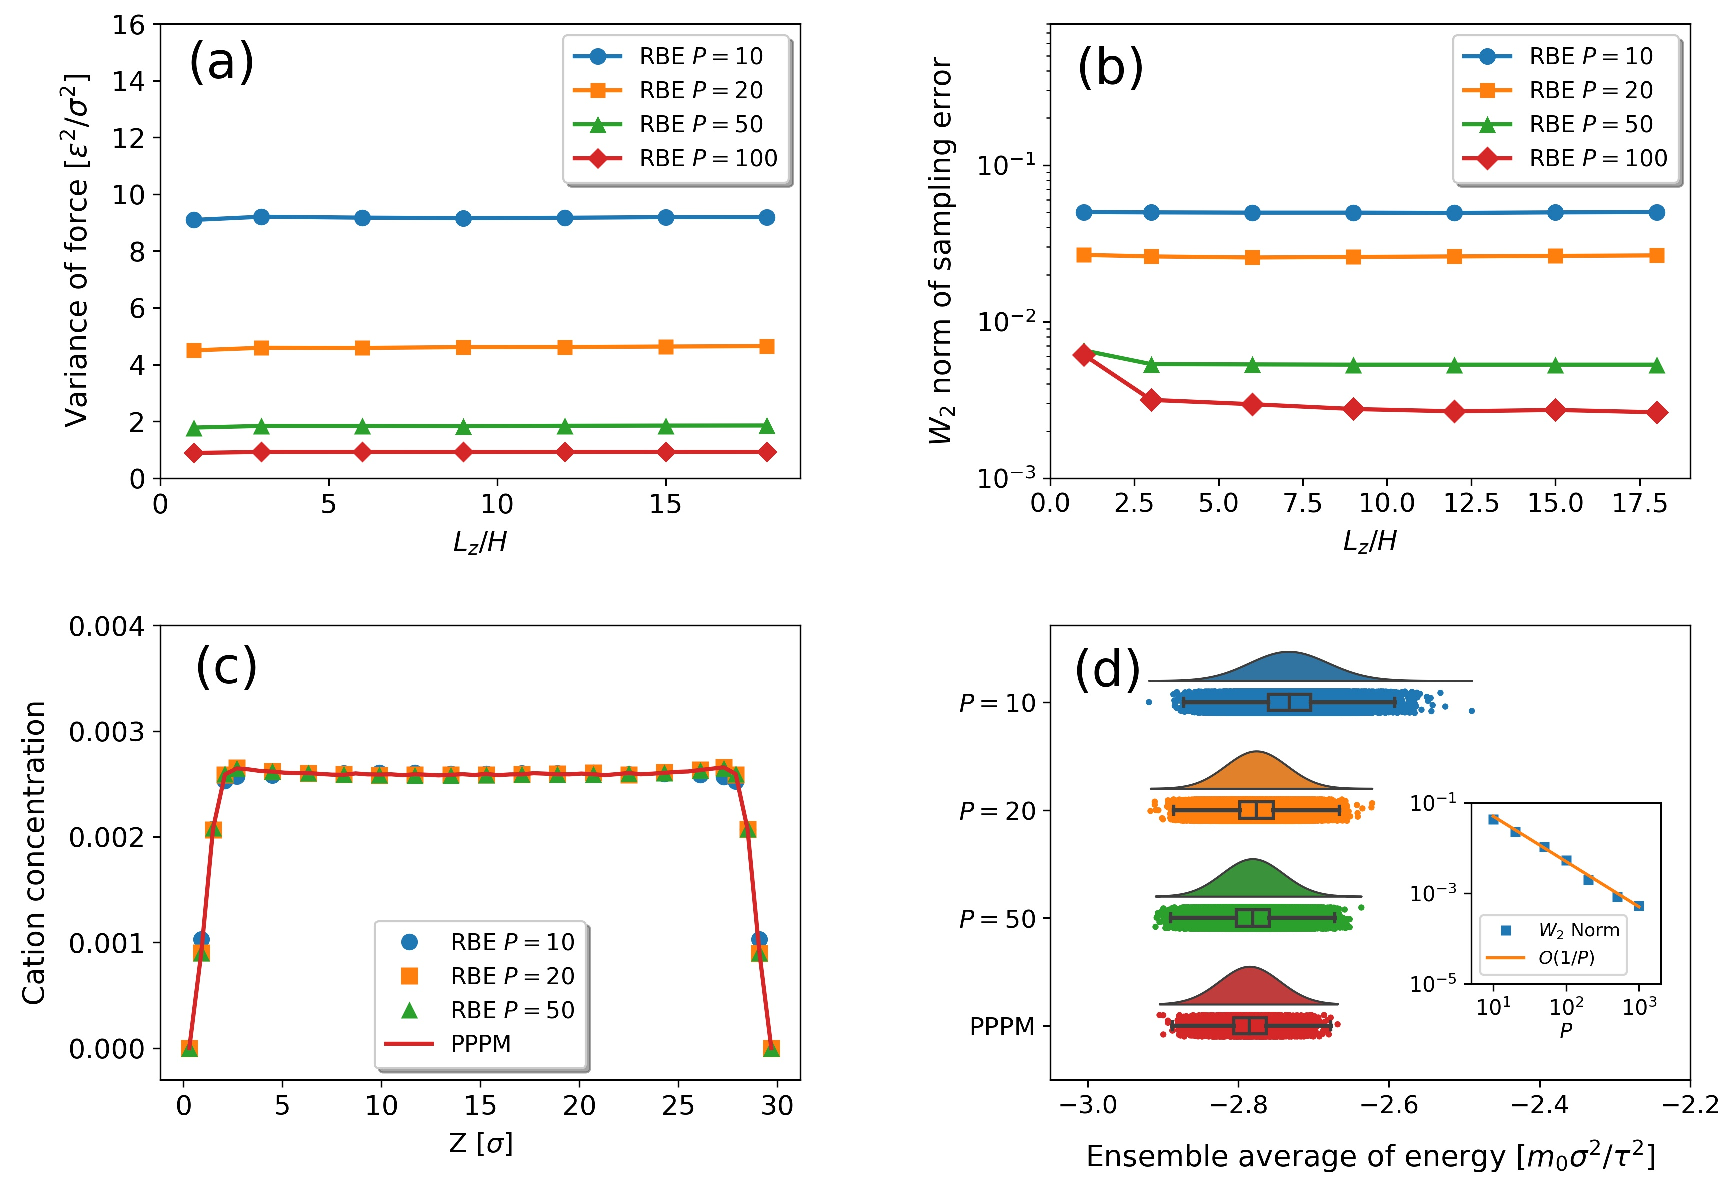
\includegraphics[width=0.90\linewidth]{figs/3_1Elec.pdf}
	\caption{MD results for $3:1$ electrolytes. (a-b):  Variance of force and the error on ensemble average of the potential energy as a function of the relative size of the extended system, $L_z/H$. (c):  Concentration of cations along $z$-dimension. (d):  Raincloud plots of the ensemble average distribution of the potential energy as well as a boxplot and raw data-points. In (a), (c) and (d), results are shown for the RBE2D with different batch size {s} $P$ and the PPPM. In (b), we use the $W_2$ norm defined in Eq.~\eqref{eq::W2} to measure the difference between two distributions. The inset in (d) shows the convergence on the $W_2$ norm with $\mathcal{O}(1/P)$ rate.}
	\label{fig:3_1}
\end{figure}

First, we consider the ensemble average of the variance in forces, denoted as $\langle\|\mathbb{E}|\bm{\Xi}_i|^2\|_{\infty}\rangle$, as shown in Fig.~\ref{fig:3_1}(a). 
Clearly, the force variance is independent   {of} the vacuum layer thickness parameter $L_z$, which validates our theoretical result stated in Theorem~\ref{Thm::1}. 
 {Then we compared the distributions of the potential energy of the obtained samples by the RBE2D and PPPM methods, denoted as~$\mathscr{P}_{\text{RBE}}(\V{x})$ and $\mathscr{P}_{\text{PPPM}}(\V{y})$, respectively.
The Wasserstein-2 norm~\cite{santambrogio2015optimal, kolbe_2024_10912241} is used to measure the difference between two distributions, defined as:}
\begin{equation}\label{eq::W2}
    W_2(\mathscr{P}_{\text{RBE}}, \mathscr{P}_{\text{PPPM}})=\left(\inf _{\gamma \in \Pi(\mathscr{P}_{\text{RBE}}, \mathscr{P}_{\text{PPPM}})} \int|\bm{x} - \bm{y}|^2 d  {\gamma(\bm{x},\bm{y})}\right)^{1 / 2}\;,
\end{equation}
where $\Pi(\mathscr{P}_{\text{RBE}}, \mathscr{P}_{\text{PPPM}})$ represents the set of all joint distributions with marginal distributions $\mathscr{P}_{\text{RBE}}$ and $\mathscr{P}_{\text{PPPM}}$.
The corresponding results are shown Fig.~\ref{fig:3_1}(b), where the~$W_2$ norms are   {plotted} as functions of~$L_z / H$ with   {varying} batch size~$P$.
According to the error estimination in Section~\ref{sec:error_reform}, when $L_z\approx H$, the errors coming from the ELC and remainder error term are still large and can not be ignored;   {this} is consistent with the error decay observed here. 
We also find that, as $L_z\geq 3H$, the error no longer decreases as $L_z/H$ increases (with $P$ fixed); indicating that
both ELC and remainder error terms now indeed become negligible, and the error primarily comes from the random batch approximation. 
%Therefore, when the batch size $P$ is fixed, the error no longer decreases as $L_z/H$ grows beyond a certain extent.


Finally, the concentration of trivalent ions along $z$ and the distribution of energy are investigated.
%with different batch sizes and $L_z/H$ fixed to be $3$, demonstrating the capability of the RBE2D to accurately reproduce the spatial structure and the ensemble averages. 
The corresponding results are depicted in Fig.~\ref{fig:3_1}(c-d). 
We observe a convergence rate of $\mathcal{O}(1/P)$ in the average energy by the RBE2D (with that of the PPPM set as benchmark value). 
This is consistent with our theoretical prediction Theorem~\ref{Thm::1} as the energies of both Coulomb and LJ scale quadratically in displacement near equilibrium.
It is also noticed that, for the RBE2D method, choosing $P=50$ can already yield very accurate results, almost indistinguishable from those obtained via PPPM. 
 {Theorem~\ref{thm::2} also indicates that the error bound in the potential energy of the RBE2D method should converge linearly in $\Delta t$. 
 As numerically validated in Fig.~\ref{fig:energy2d_3_1}, the error indeed decays with $\mathcal{O}(\Delta t)$ scaling. However, this $\mathcal{O}(\Delta t)$ scaling may not hold when $\Delta t$ is larger or in more complicated molecular models. 
 In those scenarios, increasing \(\Delta t\) can lead to particles coming very close to one another (even with the presence of the LJ potential), introducing additional sources of error in other MD components—particularly in managing bond, angle, and dihedral constraints~\cite{frenkel2023understanding}. These artificial effects may result in unphysically large forces or even cause the simulation to fail.}
%Furthermore, we observe a 

\subsection{Accuracy test case II: all-atom SPC/E bulk water system}
\label{sec::waterhomo}

%To further demonstrate the accuracy and efficiency of the proposed RBE2D method, 
Next, we perform MD simulations for the SPC/E bulk water system~\cite{berendsen1987missing}. 
The system has dimensions $L_x=L_y=H=55.9~\mathring{\text{A}}$ and consists of $17496$ atoms. 
Two purely repulsive shifted-truncated LJ walls (with $\varepsilon_{\text{atom-wall}}= k_{\text{B}}T)$ are located at $z=0$ and $z=H$. 
The simulations utilize a time step $\Delta t=1fs$, and $T$ is fixed at $298K$ by a NH thermostat with relaxation time $10fs$. 
Equilibration proceeds for $10^5$ time steps, followed by a $10^6$ steps production period, with configurations sampled every $100$ time steps. 
The cutoff is set as $r_c=10\mathring{A}$, and the ratio $L_z/H$ is fixed as $3$ to ensure that both the ELC and remainder error term are negligible.

\begin{figure}[ht!]
\centering
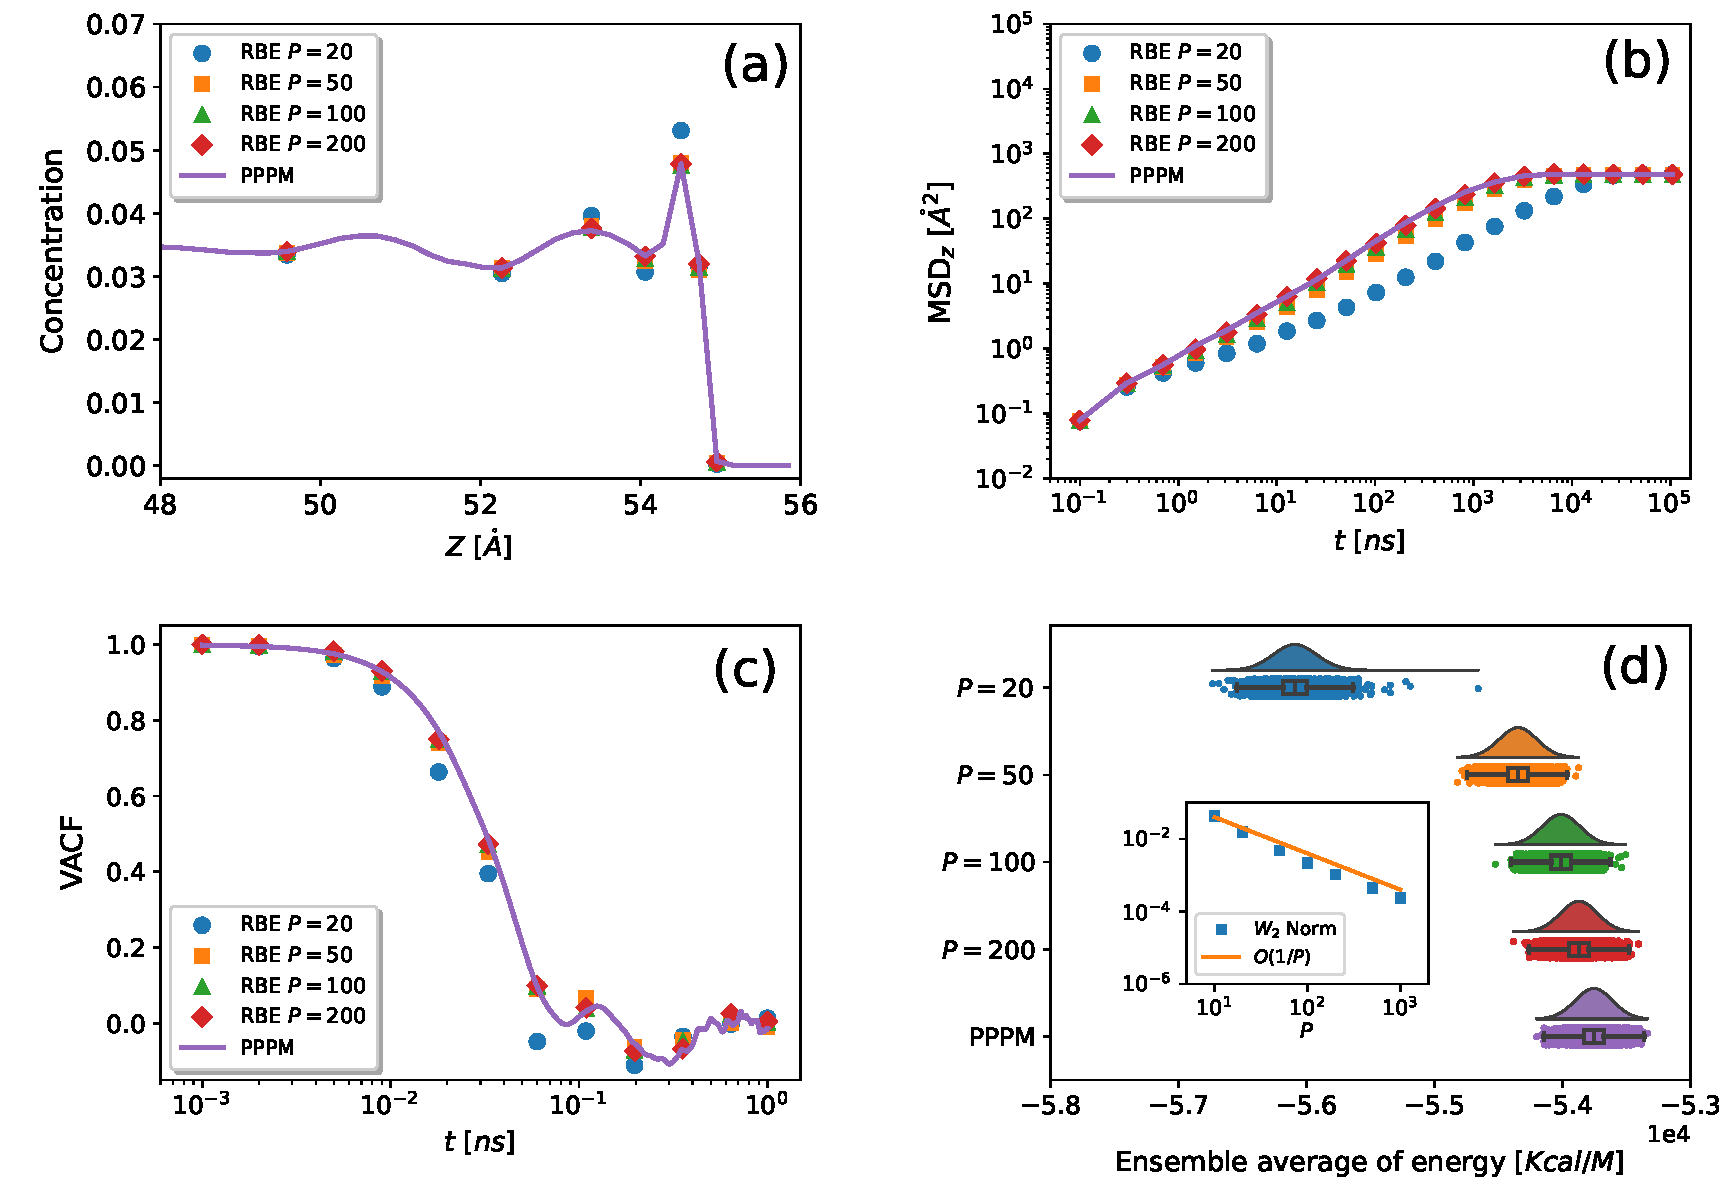
\includegraphics[width=0.90\linewidth]{figs/Density_new.pdf}
	\caption{MD results for a SPC/E bulk water system. (a)  Concentration of oxygen near the top surface; (b)  MSD along $z$-direction; (c)  VACF; and (d)  raincloud plots of the ensemble average distribution of the potential energy as well as a boxplot and raw data-points. The RBE2D with different batch size {s} $P$ and the PPPM are plotted. The inset in (d) shows the convergence on the $W_2$ norm with $\mathcal{O}(1/P)$ rate.}
	\label{fig:Water}
\end{figure}

We analyze various equilibrium and dynamic properties of the system, including the oxygen concentration, the MSD in $z$, the VACF, and the distribution of potential energy $U$.
The results are summarized in Fig.~\ref{fig:Water}(a-d).
Notably, the RBE2D method yields highly consistent results in comparison to the PPPM method across all examined properties when $P \geq 100$. 
This underscores the RBE2D's ability to effectively capture spatiotemporal information across multiple scales in molecular dynamics simulations.

\subsection{CPU time performance}
We now report the CPU time performance of the RBE2D method, compared to the PPPM method. 
The SPC/E bulk water systems are simulated, where
the system dimensions are set as $L_x=L_y=H$,  and the system size changes as one varies $N$ with the density of water being fixed at $1g/cm^3$. For a fair comparison, a cutoff of $10\mathring{A}$ and a relative error threshold of $10^{-4}$ are set for both methods.

%To ensure a fair comparison, we adopt the parameter selection strategy used in the PPPM method, establishing a relative error threshold of $10^{-4}$. For the RBE2D method, we set the Ewald splitting parameter $\alpha$ and the real space cutoff distance $r_c$ to match those of the PPPM method. Additionally, we select batch sizes of $P=100$ and $P=200$ for the RBE2D method, which have been confirmed to provide sufficient accuracy in previous sections.}
% For a fair comparison, a relative error threshold of $10^{-4}$ is set for both methods. 

\begin{figure}[ht!]
\centering	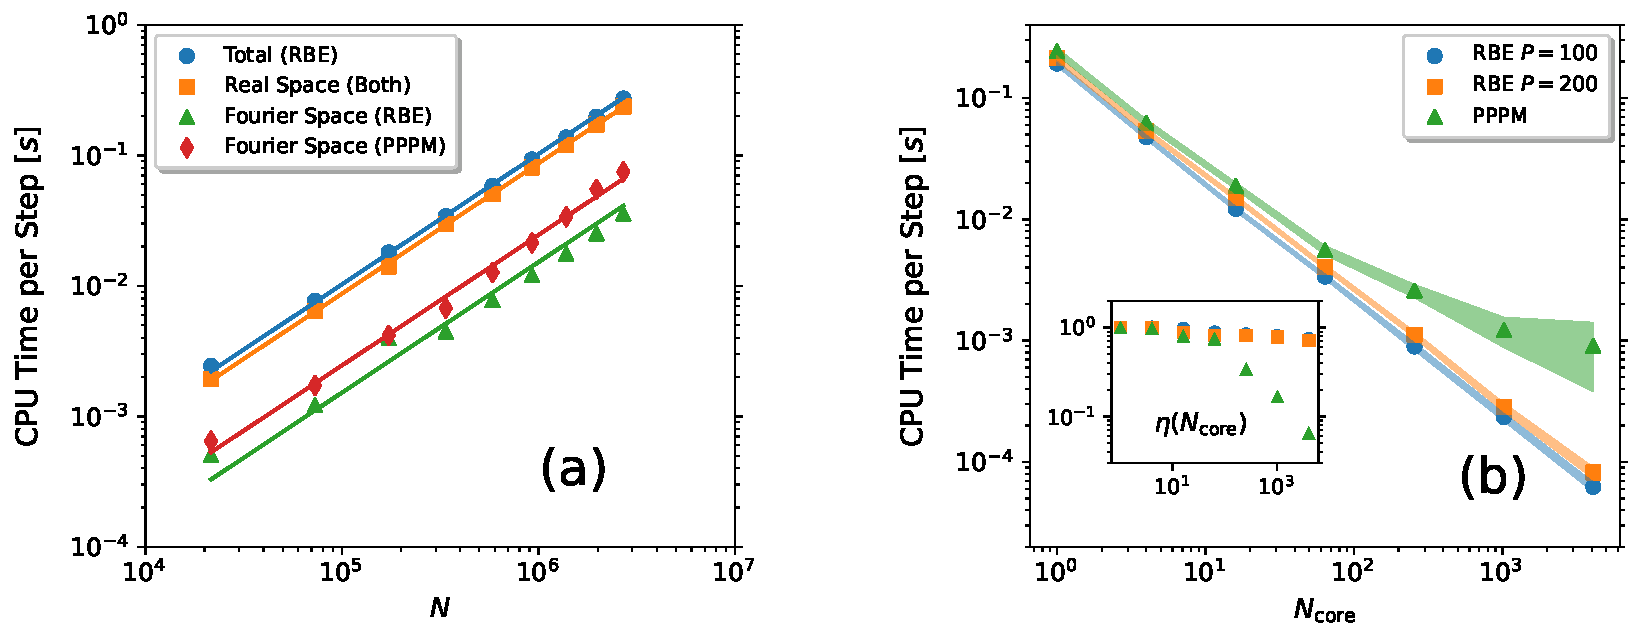
\includegraphics[width=0.9\linewidth]{figs/cpu_time_nonsub.pdf}
	\caption{
     (a) CPU time per step for the RBE2D method  {and PPPM method} with increasing $N$ and (b) total CPU time for comparison between the RBE2D and the PPPM with the number of CPU cores $N_{\emph{core}}$ up to $1024$.  {The results in (a) are obtained} with $64$ cores and $P=100$, where  {the real space cost is identical for both methods by fixing the same Ewald splitting parameter $\alpha$ and real space cutoff $r_c$.}
     The solid lines indicate linear-scaling. 
     In (b), data   {is} shown for the RBE2D with batch size $P=100$ and $P=200$ and the PPPM, where the light-colored parts stand for the range of error bar. The inset in (b) shows the   {strong parallel efficiency} $\eta(N_{\emph{core}})$.}
	\label{fig:Time}
\end{figure}

We first investigate the time cost and complexity by varying particle number $N$. 
In Fig.~\ref{fig:Time}(a), $64$ CPU cores are used, and the  CPU time per MD step for the RBE2D  {and the PPPM method} is documented with particle number $N$ up to $2\times 10^6$, where  {the real space CPU cost is identical for both methods by fixing the same Ewald splitting parameter $\alpha$ and real space cutoff $r_c$}.
 {It should be noted that the main goal of such parameter choice is for solely comparing the improvement of the RBE2D in Fourier space. We expect a fine tuning of $\alpha$ and other parameters to balance the cost of the RBE2D in real and Fourier spaces can further optimize its efficiency in practice.}
The results clearly  {demonstrate} the $\mathcal{O}(N)$ complexity of the RBE2D method  {and its significant advantage over the PPPM method in the Fourier space computation.}
 {A more detailed comparison is further provided in Fig.~\ref{fig:timenondie}, where we compared the performance of each components of the RBE2D and PPPM methods with CPU cores fixed to be both $64$ and $1024$. The results show the improvement of the RBE2D method in the Fourier component computation across the entire range of particle numbers $N$, especially when utilizing a larger number of CPU cores.} %For the PPPM method, the communication cost grows rapidly in $N_{\mathrm{cores}}$, so that the $\mathcal{O}(N\log N)$ complexity is not observed when $N_{\mathrm{cores}}=1024$.} 
%\todo{do we need a reference here}
%For  {the PPPM method}, the CPU time of the real space and the Fourier space computations are balanced to  {achieve optimal efficiency.} 
% {For the RBE2D method, in order to illustrate its advantage in reducing the Fourier space cost compared to the PPPM method, we use the same Ewald parameter $\alpha$ and real space cutoff $r_c$ as PPPM to make sure that the real space cost is identical.
% {Fig.~\ref{fig:timenondie} demonstrates that the RBE2D method significantly reduces CPU time costs compared to the PPPM method, particularly in the Fourier component across the entire range of particle numbers $N$, especially when utilizing a larger number of CPU cores.}


%demonstrating the attractive performance of the algorithm. 
% {It is important to note that the costs associated with the real space and Fourier space computations of the RBE2D method, as shown in Fig.~\ref{fig:Time}(a), are not entirely balanced. This is due to the use of the same parameters $\alpha$ and $r_c$ as those in the PPPM method for a fair comparison. The performance of the RBE2D method can be further enhanced by optimizing the parameters $\alpha$, $r_c$, and $P$.}

Next, we compare the RBE2D and PPPM methods, in terms of both
CPU time performance and  {parallel} scalability. % one of key issues limiting both system scale and time scale of MD simulations. 
%The scalability of the RBE2D method via the strong scaling, characterizing the parallel performance tuning the number of CPU cores by fixing the system size. 
Let  {$N_{\text{core}}$ be the number of cores utilized}, and $T(N_{\text{core}})$ the corresponding CPU time.  {The parallel efficiency for a strong scaling experiment is defined as}
\begin{equation}\label{eq::etau}
\eta(N_{\text{core}})=\frac{N_{\text{min}}}{N_{\text{core}}}\frac{T_{\text{min}}}{T(N_{\text{core}})},
\end{equation}
where $T_{\text{min}}=T(N_{\text{min}})$ and $N_{\text{min}}$ is the minimal number of CPU used. 
Fig.~\ref{fig:Time}(b) and its inset document the CPU time and strong scaling results by the RBE2D and PPPM methods, for a system comprising $139968$ atoms. Clearly,
the two methods perform similarly when $N_{\text{core}}$ is small; and RBE2D outperforms PPPM as $N_{\text{core}}$ increases, the advantage becomes significant for $N_{\text{core}}>64$. Notably,
when $N_{\text{core}}\geq 1024$, RBE2D is approximately 10 times faster than PPPM. 
Furthermore, the strong scaling of the RBE2D remains over $70\%$ when~$\sim 4000$ CPUs are employed, while that of the PPPM drops raplidly to $6\%$. 
 {The main difference between these two methods lies in their communication cost. The RBE2D requires only a single global communication for the reduction of $P$ structure factors. In comparison, the PPPM method, due to its use of FFT, requires six sequential rounds of communication to perform both forward and backward Fourier transforms, leading to poor scalability~\cite{fftscalability,arnold2013comparison}.} This highlights the excellent parallel scalability of the RBE2D method. 
%Due to its mesh-free nature, the RBE2D method is expected to exhibit even greater advantages when applied to systems with strong confinement, where $H\ll\min\{L_x,L_y\}$. In such cases, the PPPM method requires more meshes, leading to a loss in efficiency. 


\section{Numerical results on quasi-2D systems under dielectric confinement}\label{sec::numericalDielectric}

In this section, numerical simulations are performed for systems in the presence of dielectric interfaces, including dielectrically confined electrolytes and SPC/E bulk water, to further validate the RBE2D method.  {Reduced LJ units and real units are used to parameterize these systems, respectively.}
As a benchmark for accuracy and efficiency, the simulations are also  conducted using the HSMA method~\cite{liang2020harmonic} and the ICM-PPPM method~\cite{yuan2021particle}, both have been implemented in LAMMPS~\cite{liang2022hsma}. 
For the RBE2D, parameters such as $M$ and $L_z$ are selected according to Section~\ref{sec:parameter}; while
for the HSMA and ICM-PPPM, we use the same parameters suggested by Refs.~\cite{liang2020harmonic} and~\cite{yuan2021particle}, respectively. For all methods, the threshold in  relative errors is set to $10^{-4}$.

\subsection{Accuracy test case III: dielectrically confined electrolytes}

%To demonstrate the accuracy of the RBE2D method in MD simulations with planar dielectric 
Here we examine four distinct electrolyte systems that are confined by two dielectric interfaces.
These systems include 2:1 and 3:1 electrolytes with varying surface charge densities and dielectric contrasts.
In these systems, all ions are modeled as soft spheres of diameter $r_{\text{d}}$, and are confined by purely repulsive shifted-truncated LJ walls ($\varepsilon_{\text{ion-wall}}=k_{\text{B}}T$; $\sigma_{\text{ion-wall}}=0.5r_{\text{d}}$) at $z=0$ and $z=H$. More detailed information regarding the system settings can be found in Table~\ref{Table::Dielec}.
The MD simulations utilize a time step $0.005\tau$, with temperature controlled by a NH thermostat %using an external temperature of $T=1$ and 
with a damping time of $0.05\tau$,  {where $\tau$ is the reduced LJ unit of time defined in Section \ref{subsec::electrolyte-neutral}}.
All simulations start with an equilibration period of $10^6$ time steps, followed by a production period of $10^8$ time steps.

\begin{figure}[ht!]
\centering
	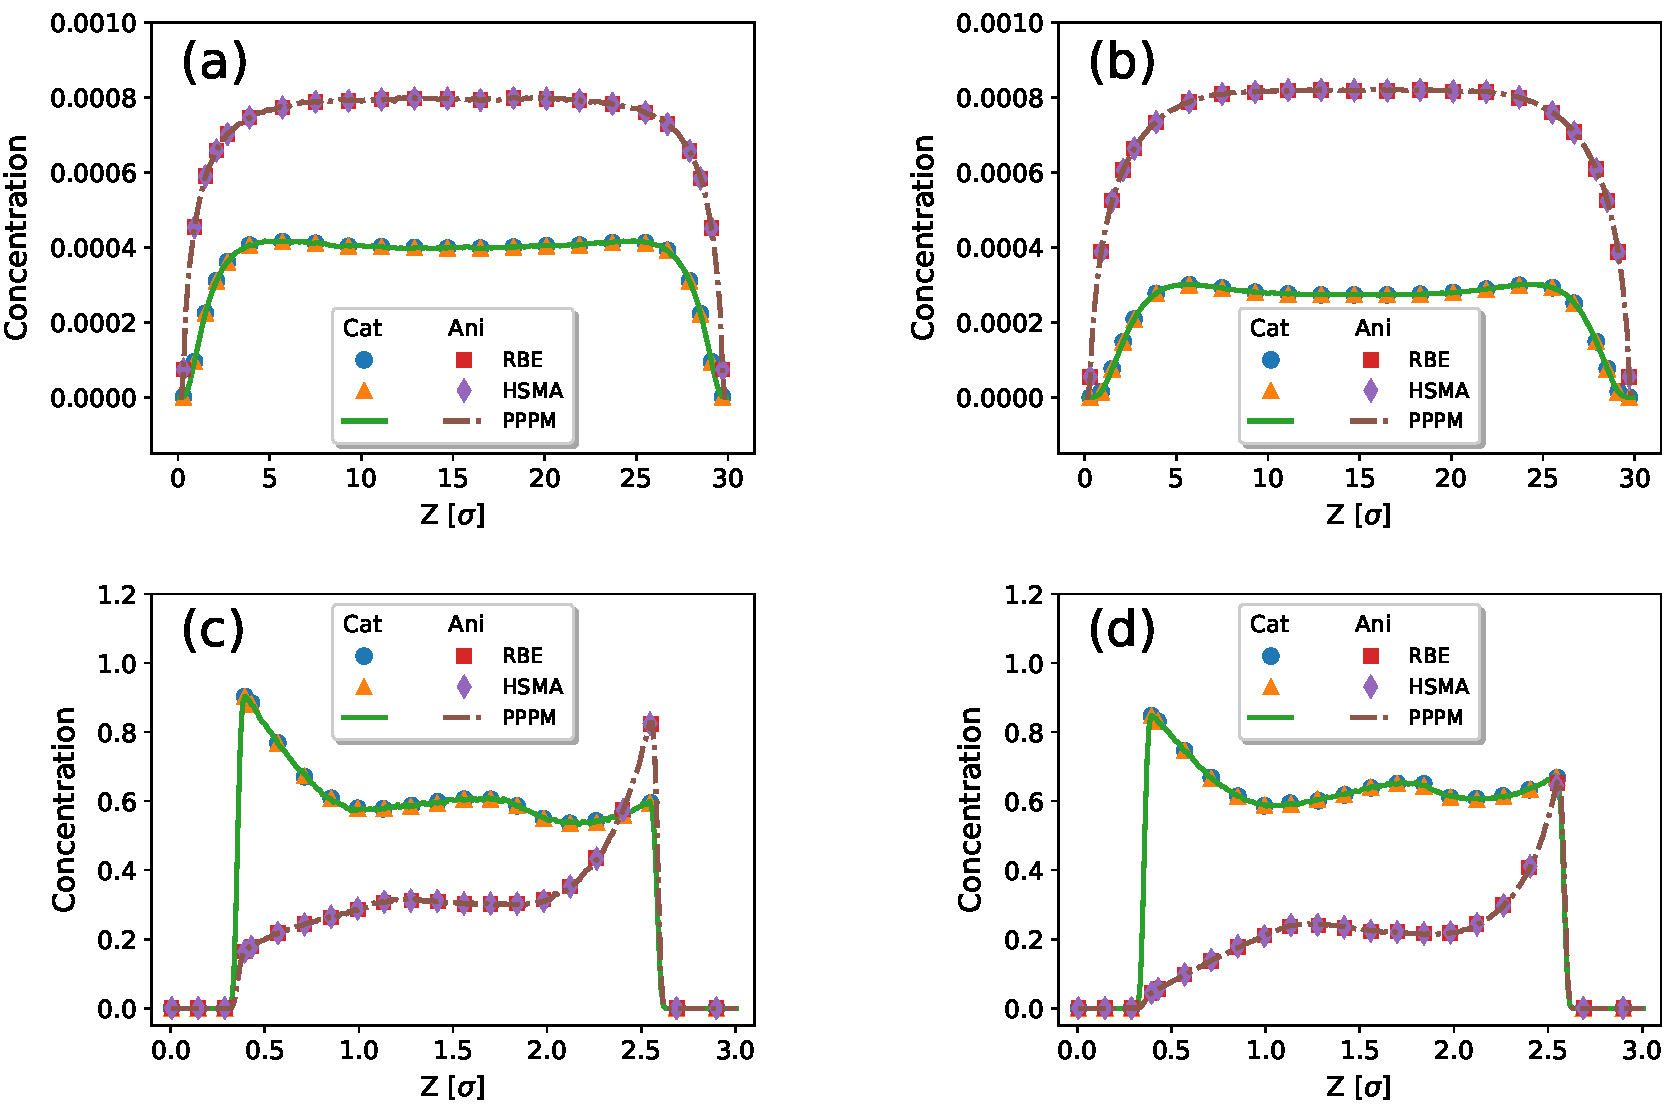
\includegraphics[width=0.95\linewidth]{figs/DistributionDie.pdf}
	\caption{Ionic distributions for [(a) $2:1$ electrolyte and (b) $3:1$ electrolyte] between neutral interfaces with symmetric dielectric contrast, and [(c) $2:1$ electrolyte and (d) $3:1$ electrolyte] confined between walls with asymmetric dielectric contrasts and non-neutral asymmetric surface charge densities. More details about the system settings are provided in Tab.~\ref{Table::Dielec}. 
    Data   {is} shown for the RBE2D method with batch size $P=100$, and the HSMA and the ICM-PPPM methods with relative error threshold $10^{-4}$.} 
	\label{fig:den1}
\end{figure}

We first calculate the cation and anion distributions along  {the} $z$-axis for all considered systems, the results are summarized in Figure~\ref{fig:den1}(a-d). 
In panels (a-b), where the dielectric contrasts are set as $\gamma_{\text{top}}=\gamma_{\text{bot}}=0.939$, the concentrations illustrate the so-called ``ion depletion effect'' near the insulator-like interfaces, consistent with previous findings. 
%In panels (C-D), it is observed that the presence of surface charge modulates this repulsive effect, with the modulation arising from the addition of counterions to maintain charge neutrality. 
Panels (c-d) demonstrate the complicated interplay between the dielectric confinement effect, interfacial charges, and ion valences, and their accumulative effects on the cation distribution. %while these effects mutually reinforce each other for the anion distribution.
For all cases considered, the RBE2D results show excellent agreement with that of the HSMA and ICM-PPPM methods. 
%A comparison with the HSMA and ICM-PPPM methods shows excellent agreement with the RBE2D results. 
The ion distribution shown in panel (c) also agrees with the result from a boundary element solver~\cite{wu2018asymmetric}, and reported in \cite{yuan2021particle}, figure 4(b). 
Additionally, we calculate the potential energy distribution $\mathscr{P}(U)$ for these systems and measure the discrepancy using the $W_2$ norm.
A convergence rate of $\mathcal{O}(1/P)$ is again observed (see Fig.~\ref{fig:energy2d}).

\subsection{Accuracy test case IV: dielectrically confined SPC/E Water}

%To further assess the comparison of both the accuracy and efficiency between the RBE2D and ICM-PPPM methods, 
We conclude the numerical tests with simulations of dielectrically confined SPC/E bulk water, and cross compare the RBE2D and ICM-PPPM methods. 
%The equilibrium temperature is set to $T=298K$. 
%The equilibration process was carried out for $50 ns$, followed by MD simulations on the NVT ensemble of $100ns$ for data collecting. 
One can refer to Sec.~\ref{sec::waterhomo} for most of the system setups.
Here the dielectric mismatches are introduced, set as $\gamma_{\text{top}}=\gamma_{\text{bot}}=-0.5$. 
The parameters of the ICM-PPPM method were automatically chosen~\cite{kolafa1992cutoff} to achieve a relative error of $\Delta=10^{-4}$, and the real space cutoff distance $r_c$ was set to $12\mathring{A}$, which was selected to optimize the performance of the ICM-PPPM method. 

\begin{figure}[ht]
\centering
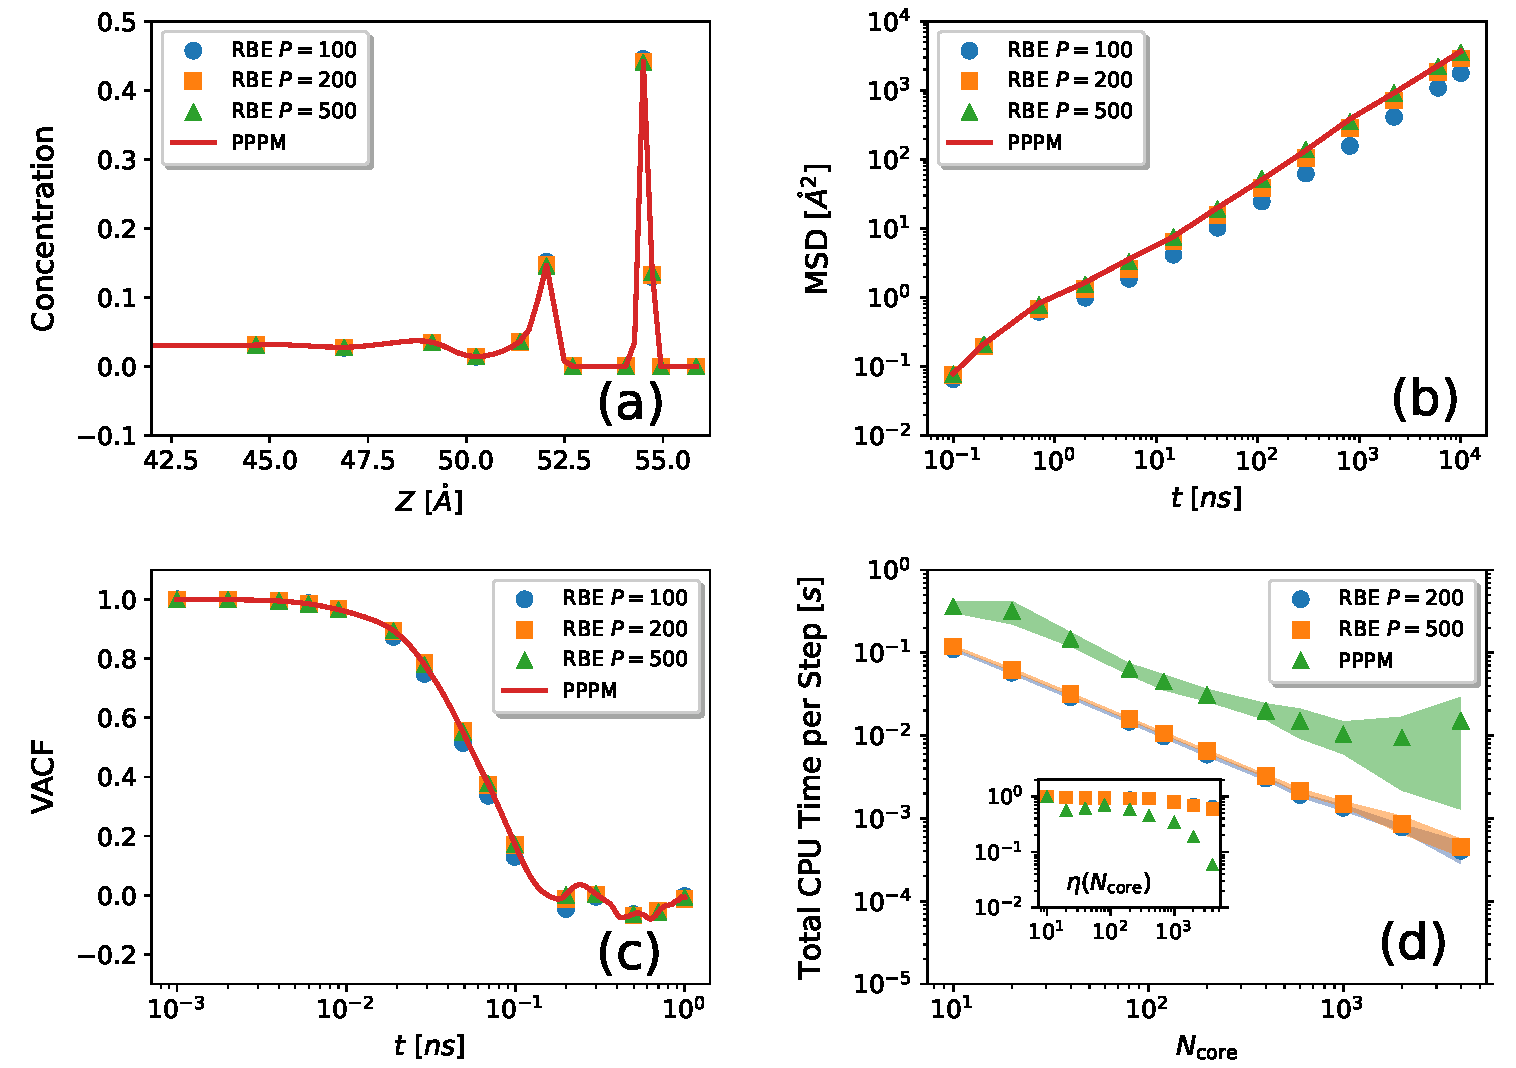
\includegraphics[width=0.95\linewidth]{figs/Dielectric.pdf}
    \caption{Distribution of oxygen atom {s} in SPC/E bulk water system (a), the MSD (b), the VACF (c), and comparison of time performance between RBE2D (with different $P$) and ICM-PPPM (d) are studied. 
    The inset in (d) shows  {the} corresponding strong parallel efficiency $\eta(N_{\text{core}})$ defined as Eq.~\eqref{eq::etau}. 
    The results derived from the RBE2D   {are} almost identical to those from the ICM-PPPM. 
     {The RBE2D based MD is about $1.5$ orders of magnitudes faster than the ICM-PPPM-based MD.}
    }
    \label{fig:den2}
\end{figure}

We first examine the concentration of oxygen along  {the} $z$-axis for a system comprising $53367$ atoms, the results are displayed in Fig.~\ref{fig:den2}(a). 
We again find  excellent agreement between the RBE2D and the ICM-PPPM when $P\geq 200$, whereas some small discrepancy is observed if one chooses $P=100$. 
The MSD and VACF are also calculated and shown in Figs.~\ref{fig:den2}(b-c).
The results clearly indicate that for dynamic properties of the water molecules (such as MSD and VACF), the results obtained by RBE2D is consistent   {with} that of the ICM-PPPM  {across} multiple time scales ($fs$ to $ns$). 

Finally, the CPU time and scalability data of both the RBE2D and ICM-PPPM methods are documented in Fig.~\ref{fig:den2}(d), based on simulating a water system containing $139968$ atoms. It is observed that, the RBE2D is more than 10 times faster than the ICM-PPPM method. 
Furthermore, the   {parallel efficiency} is shown in the inset of Fig.~\ref{fig:den2}(d), which indicates that RBE2D can remain a strong scaling of $60\%$ for up to $4000$ CPU cores, while that of ICM-PPPM drops to only about $5\%$, again demonstrating the strong   {parallel efficiency} of RBE2D method.  {We also provide a more detailed comparison between the RBE2D and ICM-PPPM methods in Fig.~\ref{fig:timedie} in the SM, using the same number of CPU cores (\( N_{\text{core}} = 64 \) and 1024) and a batch size of \( P = 200 \), with varying particle number $N$. 
The results clearly demonstrate that the RBE2D outperforms the ICM-PPPM across the range of \( N \) up to \( 10^6 \).}